%%%%%%%%%%%%%%%%%%%%%%%%%%%%%%%%%%%%%%%%%%%%%%%%%%%%%%%%%%%%%%%%%%%%%%%%%%%%%%%%
% backgrounds.tex
%%%%%%%%%%%%%%%%%%%%%%%%%%%%%%%%%%%%%%%%%%%%%%%%%%%%%%%%%%%%%%%%%%%%%%%%%%%%%%%%
\chapter{Backgrounds}
\label{backgrounds}
There are several ways that standard model physics processes could mimic signal events, and the expected rate of these processes must be understood in order to meaningfully interpret the number of observed events in the signal regions in data as a limit on the signal strength of new processes.
Wherever possible, the backgrounds are determined using control regions in data where orthogonal selections to the signal region are applied in order to find regions enriched in backgrounds to study their properties and extrapolate their rate to the final selection.
By using data-driven methods, the background rates can be predicted without uncertainty from differences in simulated and data events. 
However, control regions which can effectively isolate background processes and be extrapolated into the signal region without significantly altering the event topology are not always available, and so some backgrounds must be predicted using MC and validated using data to limit effects from uncertainties in the simulation method.

Heuristically, the backgrounds in this search are split into two types: those where the probe track is produced by a muon ("muon backgrounds") and those where it is produced by any other particle in the event ($\mu+X$ events).
In practice, the invariant mass of the tag/probe pair is the primary feature used to distinguish events with non-muon probes, as muon-system and calorimeter information are heavily used in the signal definition and therefore unavailable for simple definitions of control regions.
As a result, the $\mu+X$ backgrounds include any processes where the invariant mass of the tag and probe pair does not peak near the Z-mass, effectively serving as a background of events where the probe does not originate directly from a DY muon.
While muons from other sources could potentially produce signal events in the same manner as muons from Z bosons, their much smaller relative rates causes their inclusion as backgrounds to have a negligible impact on the resulting signal sensitivity.

\section{DY Muon Backgrounds}
Standard model DY backgrounds occur when the base event selection successfully finds a probe track which matches to a muon originating from the DY process which then passes the signal selection without undergoing a Dark Bremsstrahlung. 
This can occur either when muons lose energy via conventional physics interactions without producing enough visible energy in the detector to reject the event or when the muon signature in HE and the CSC chambers is missed.
Often, some combination of both effects is present, as muons with altered energy from interactions within the detector can have genuine deflections causing them to pass through unexpected stations in the muon chambers, greatly increasing the probability of reconstructing them poorly.

The primary difficulty of muon backgrounds is the lack of control regions enriched in DY muons which do also efficiently reject signal events.
Like signal events, muon backgrounds have opposite-sign tag and probe pairs, and have nearly identical distributions of invariant mass, track isolation, and muon kinematics.
Muon backgrounds tend to have slightly higher HCAL energy deposits along the track trajectory than signal events, as muons with large energy loss to SM particles have lower energies and therefore reduced cross sections for \dbrem.
Unfortunately, events with large HCAL deposits have correspondingly large rates of SM Bremsstrahlung, which produces genuine muon deflections and significantly alters the observed behavior within the muon chambers.
As a result, the control regions with large HCAL energy near the probe track are useful for validating the performance of the muon chamber behavior for signal-like events, but cannot be used to directly extrapolate a background rate into the signal region. 

Due to the difficulty in defining control regions without significant signal contamination or large differences from the signal selection, the muon background rate for both complete and partial disappearance events is predicted using MC, and several validation studies are performed to confirm that the features used to define missed and deflected muons in simulation closely match those seen in data.
For the complete disappearance region, control regions containing fully reconstructed muons are used to predict the probability of a muon failing to produce a muon segment in any given muon chamber, and corrections are derived for differences observed between data and simulation.

For partial disappearance events, control regions with large energy deposits in HCAL aligned with probe tracks are used to validate the reconstruction of standalone muons in events with deflected muons.
The high-HCAL-energy region is also used to validate the performance of the BDT on data events and the simulated rate of SM muon Bremsstrahlung.
Additionally, events with low BDT scores are used to validate the simulation of non-signal-like muons as well as the performance of the BDT in scoring them.

\subsection{Missed Muons}
\label{sec:missedMuons}
In complete disappearance events, muon backgrounds may pass the signal selection by having the muon fail to produce hits in any CSC station due to poor reconstruction. 
These 'missed muon' events can potentially be caused by inefficient CSC stations, gaps in the detector, or physics process that deflect the muon sufficiently to pass the nearby CSC hit requirements without depositing enough energy in the calorimeters to fail the isolation requirements. 
This background is predicted using simulation, with an additional correction factor applied using studies of CSC hit reconstruction efficiency in data. 

Because the isolation requirements applied in the probe track selection result in very few non-muon tracks, the rate of missed muons should depend only on the kinematics of the selected track and otherwise be independent of the initial process which created the muon. 
The DY process produces the vast majority of selected muons, so only simulated events produced from Z decays are used to determine the rate of missed muon backgrounds.
This approach does not separate muon backgrounds from SM scattering within the HCAL and missed muon segments caused by poor reconstruction, as both effects are included in the detector response simulation.

To account for potential differences in the efficiency of the simulated CSC responses with respect to the real detector, corrections are applied to the simulated events based on the position-dependent CSC reconstruction efficiency measured using control regions containing CSC hits aligned with fully reconstructed muons.
While these muons are required to have at least two muon segments along their trajectories as part of their initial identification, the other CSC stations they pass can be used to determine the efficiency of muons producing CSC hits at the locations they traverse.
The rate of finding a muon segment within $\Delta$R$<$0.05 of the muon trajectory is measured for each CSC station as a function of $\eta$ and $\phi$, and the ratios of the measured efficiencies in data and simulation are taken to identify regions which have differences between the real and simulated detectors.
The CSC reconstruction efficiencies for data and MC as a function of $\eta$ and $\phi$ are shown in \Cref{fig:CSCeff} and \Cref{fig:CSCeff2}.

\begin{figure}[htbp]
    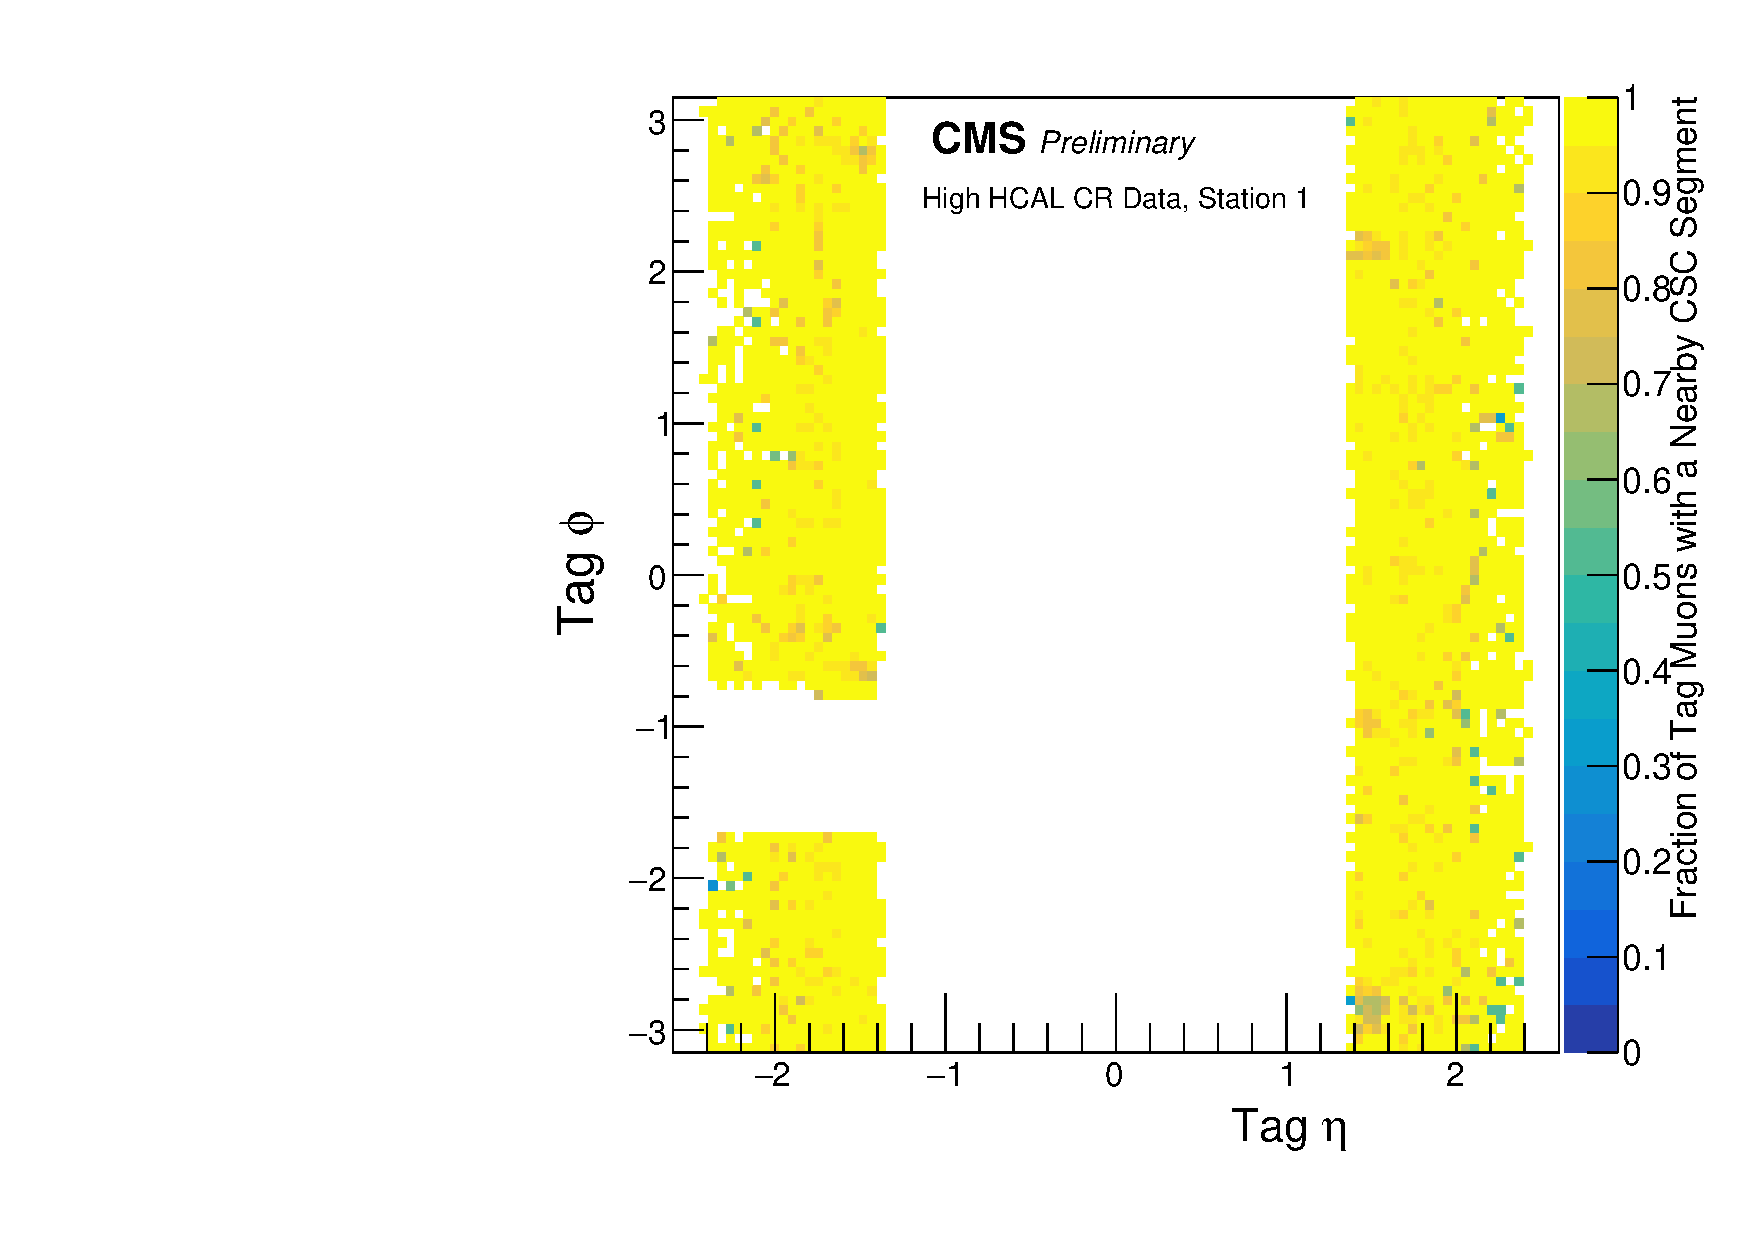
\includegraphics[width=0.45\textwidth]{figures/cscNearbyFracData_station0.pdf}
    \hspace{0.01\textwidth}
    \centering
    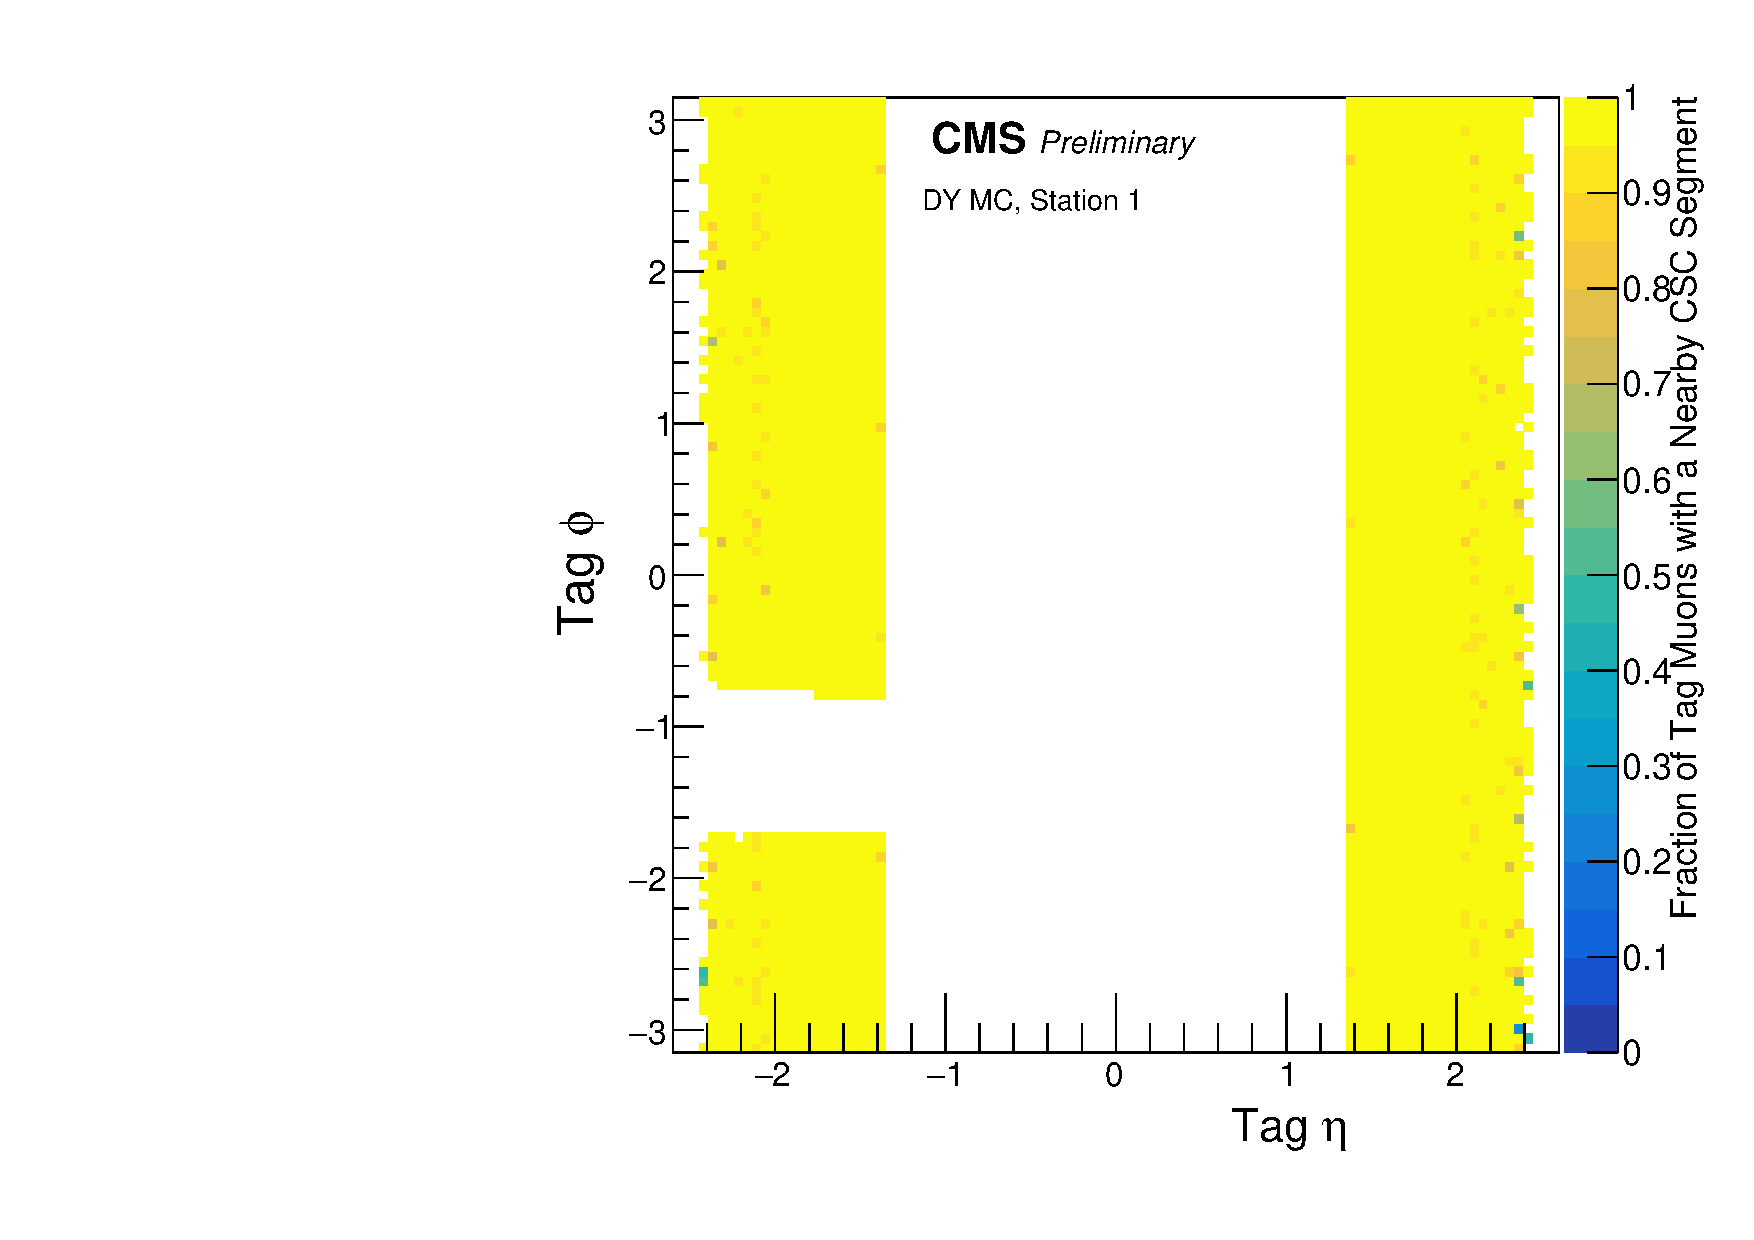
\includegraphics[width=0.45\textwidth]{figures/cscNearbyFracMC_station0.pdf}
    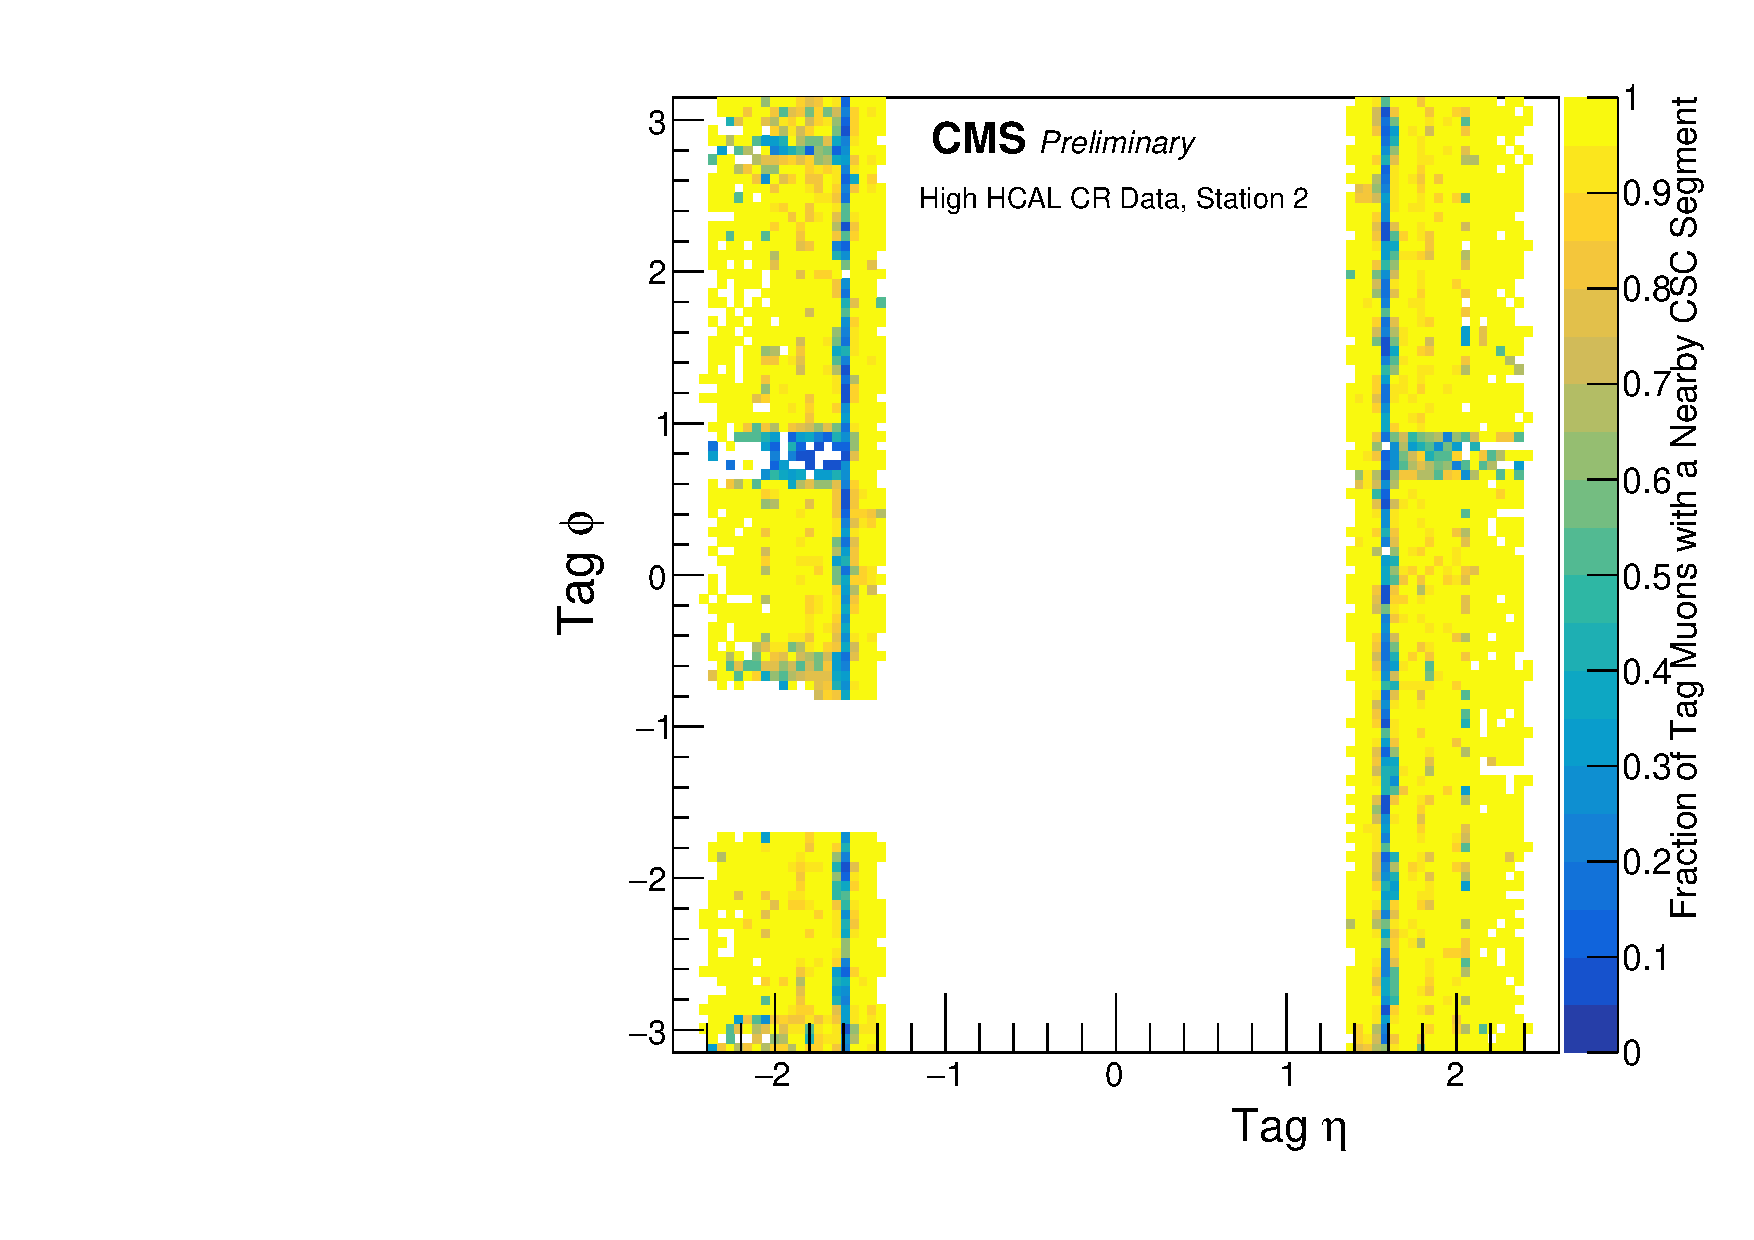
\includegraphics[width=0.45\textwidth]{figures/cscNearbyFracData_station1.pdf}
    \hspace{0.01\textwidth}
    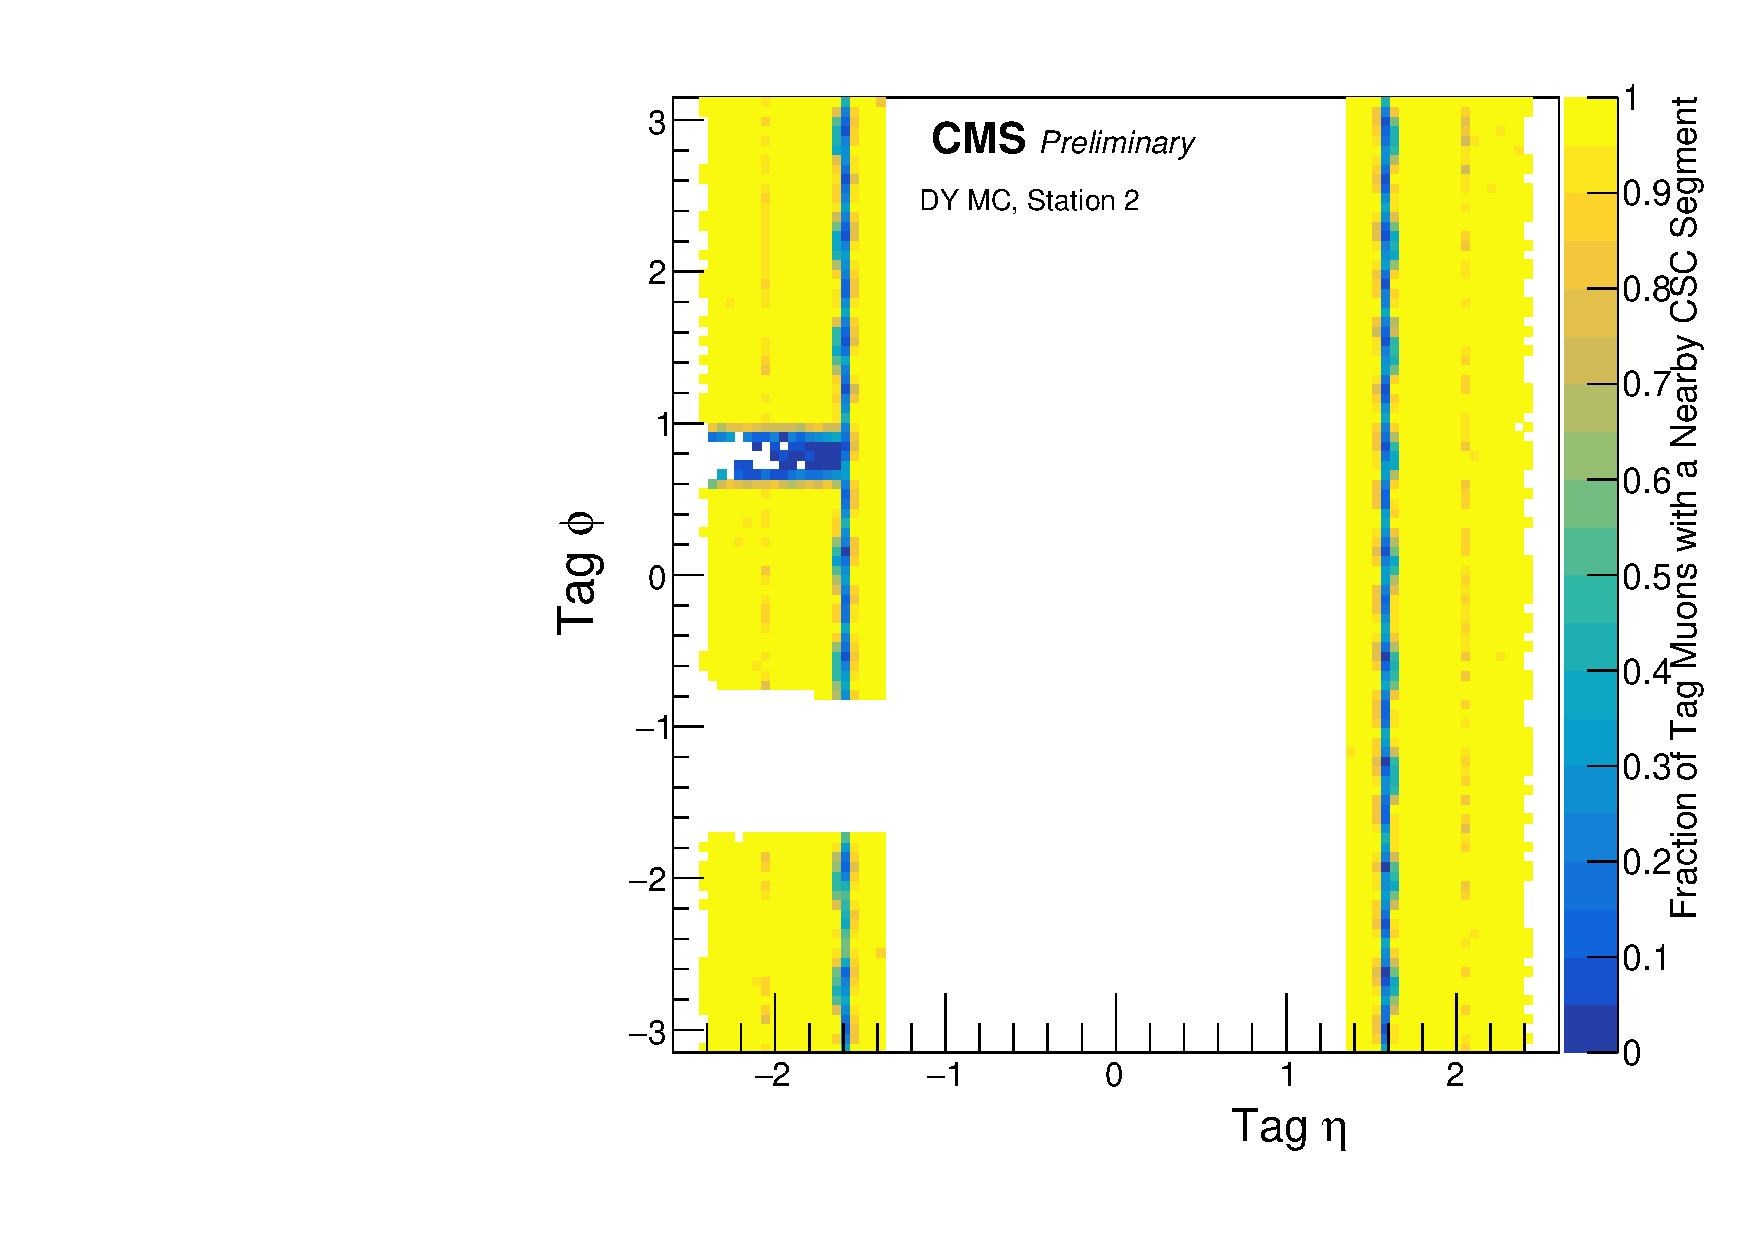
\includegraphics[width=0.45\textwidth]{figures/cscNearbyFracMC_station1.pdf}
	\caption[CSC segment efficiencies for stations one and two]{The fraction of tag muons with nearby CSC hits in the first and second CSC stations for data and MC. While the overall rate of stations with no nearby CSC hits sees good agreement across most depths, there are several locations in data that have poorer reconstruction than simulation, such as the inefficient wedge in station two near $\phi$=1,$\eta$=2. These regions are included in the complete disappearance region by removing CSC hits in MC which occur within them with event weights corresponding to the difference in reconstruction efficiency.}
    \label{fig:CSCeff}

\end{figure}
\begin{figure}[htbp]
    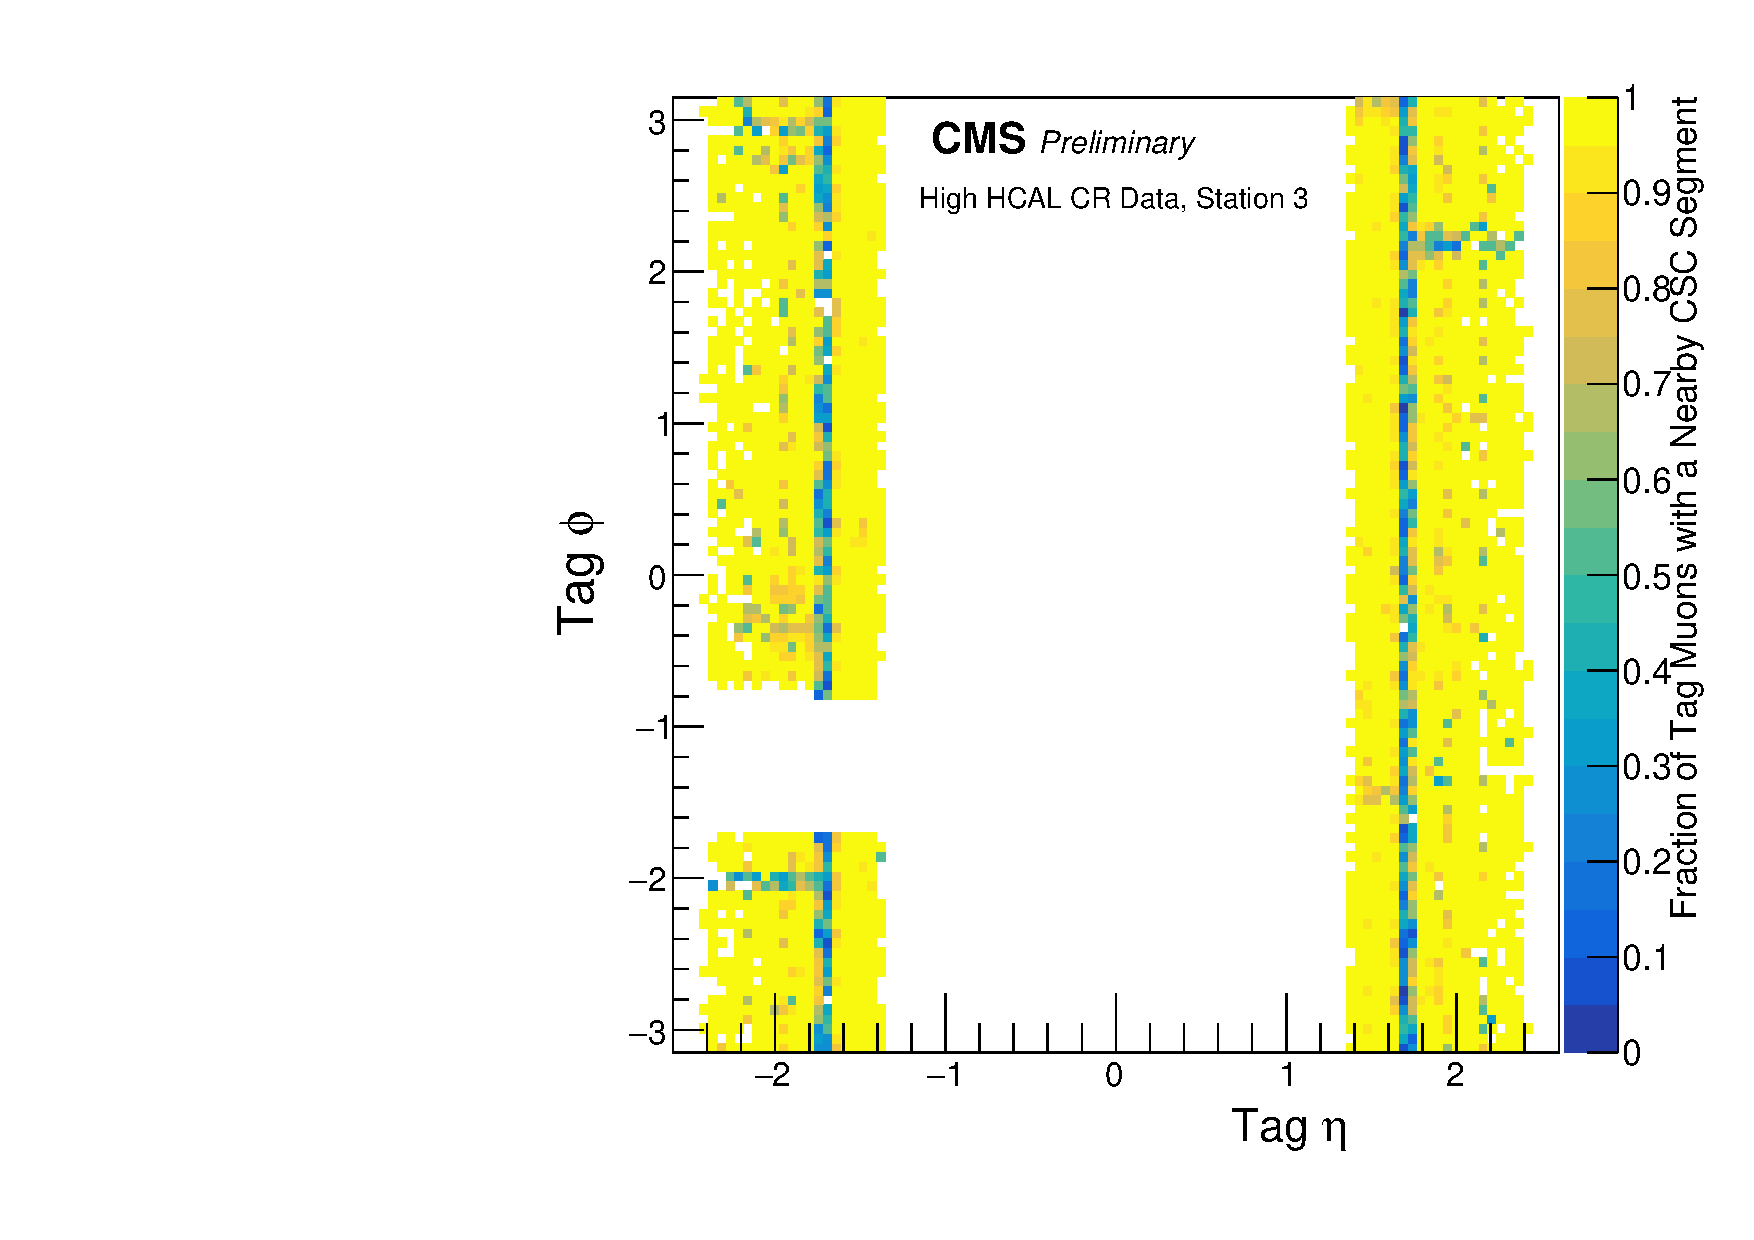
\includegraphics[width=0.45\textwidth]{figures/cscNearbyFracData_station2.pdf}
    \hspace{0.01\textwidth}
    \centering
    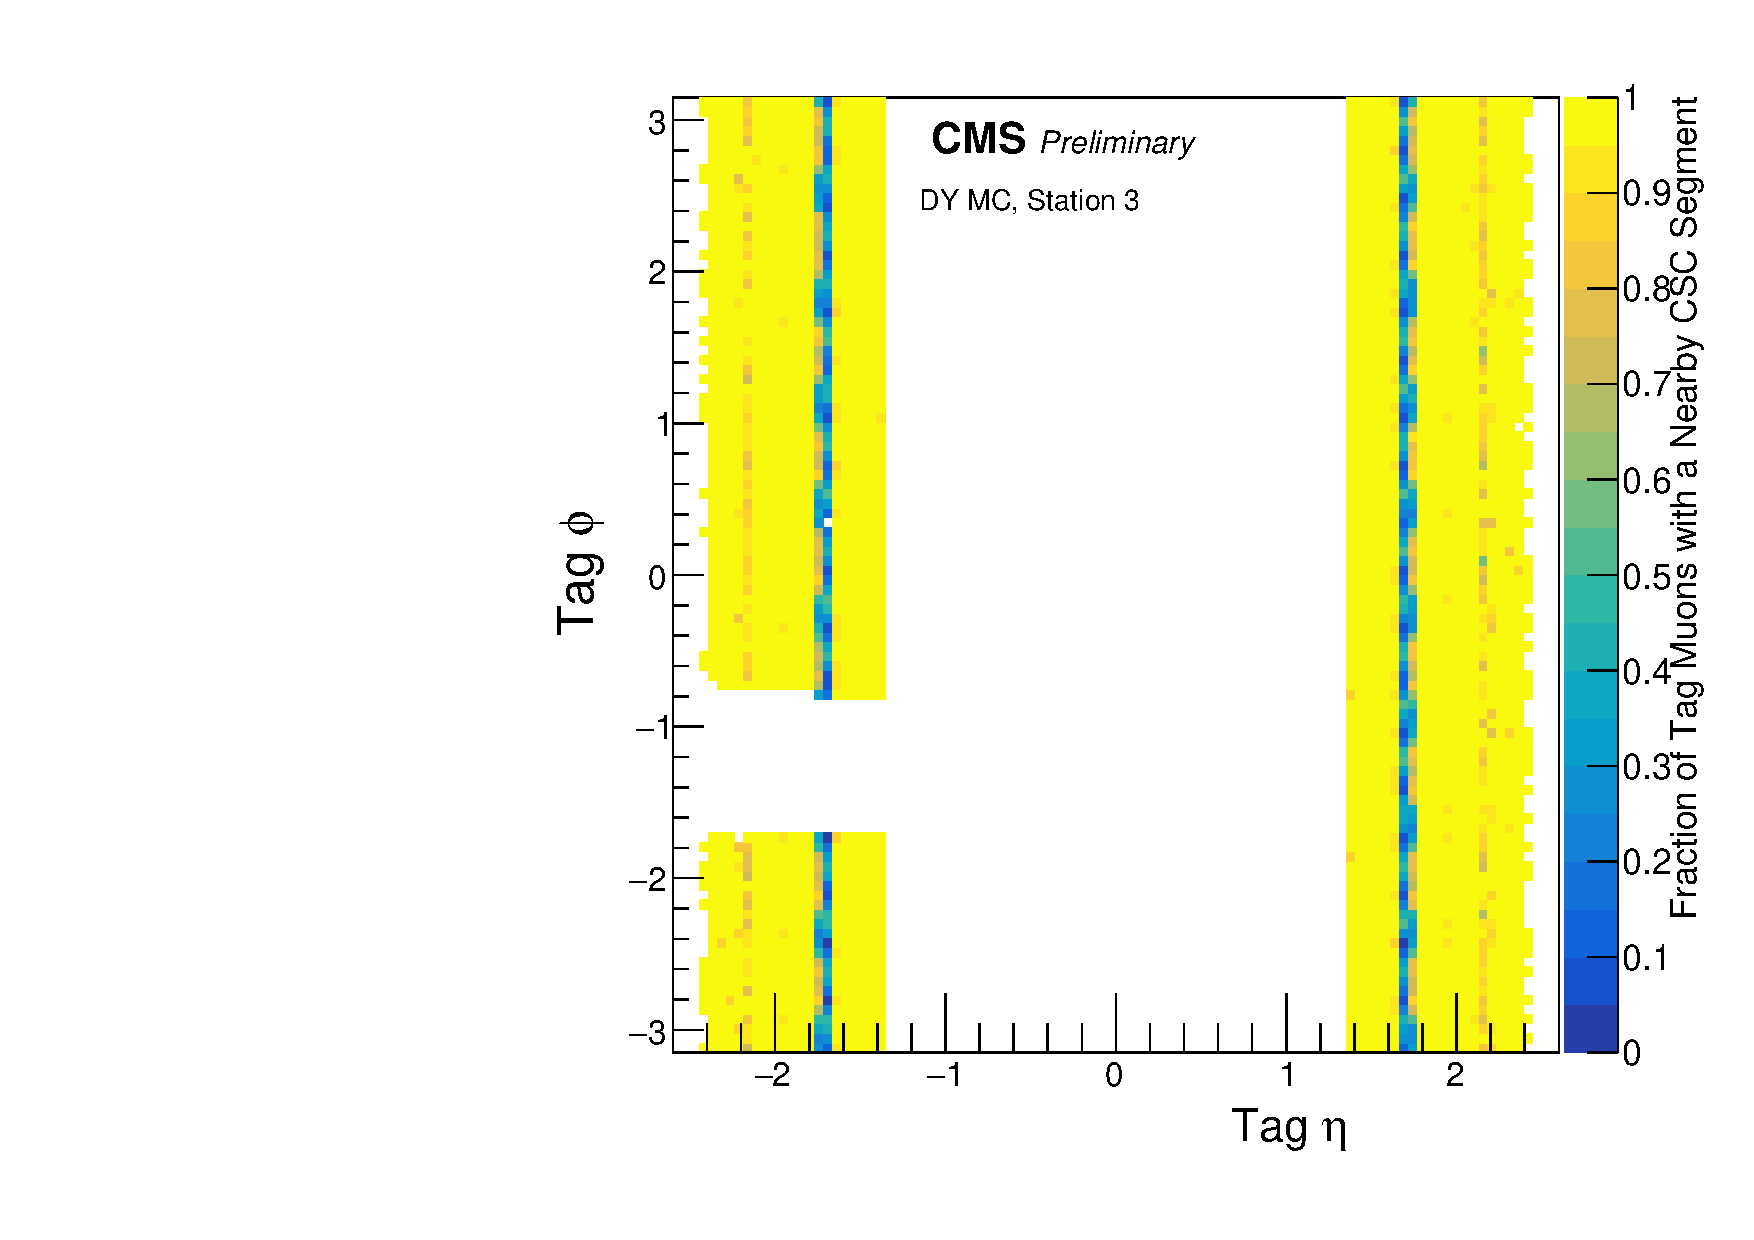
\includegraphics[width=0.45\textwidth]{figures/cscNearbyFracMC_station2.pdf}
    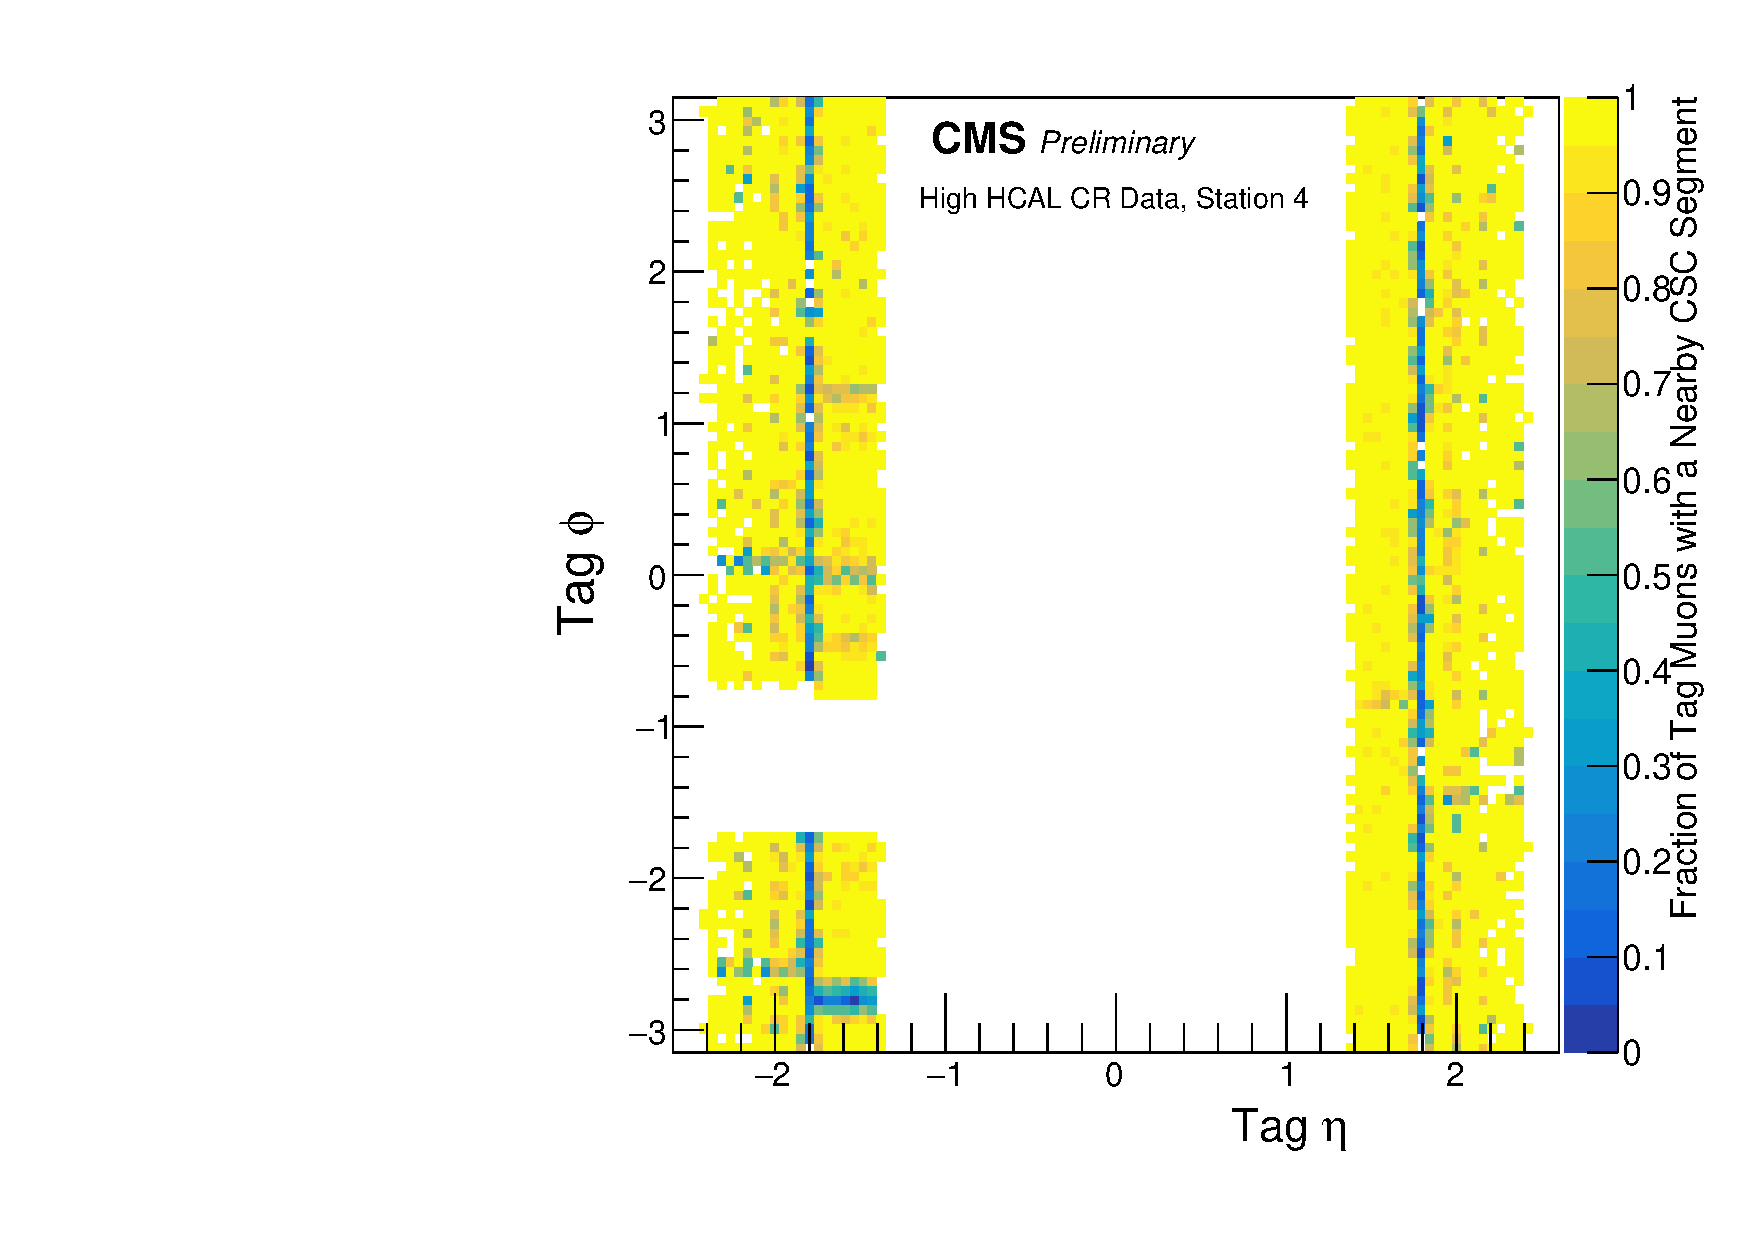
\includegraphics[width=0.45\textwidth]{figures/cscNearbyFracData_station3.pdf}
    \hspace{0.01\textwidth}
    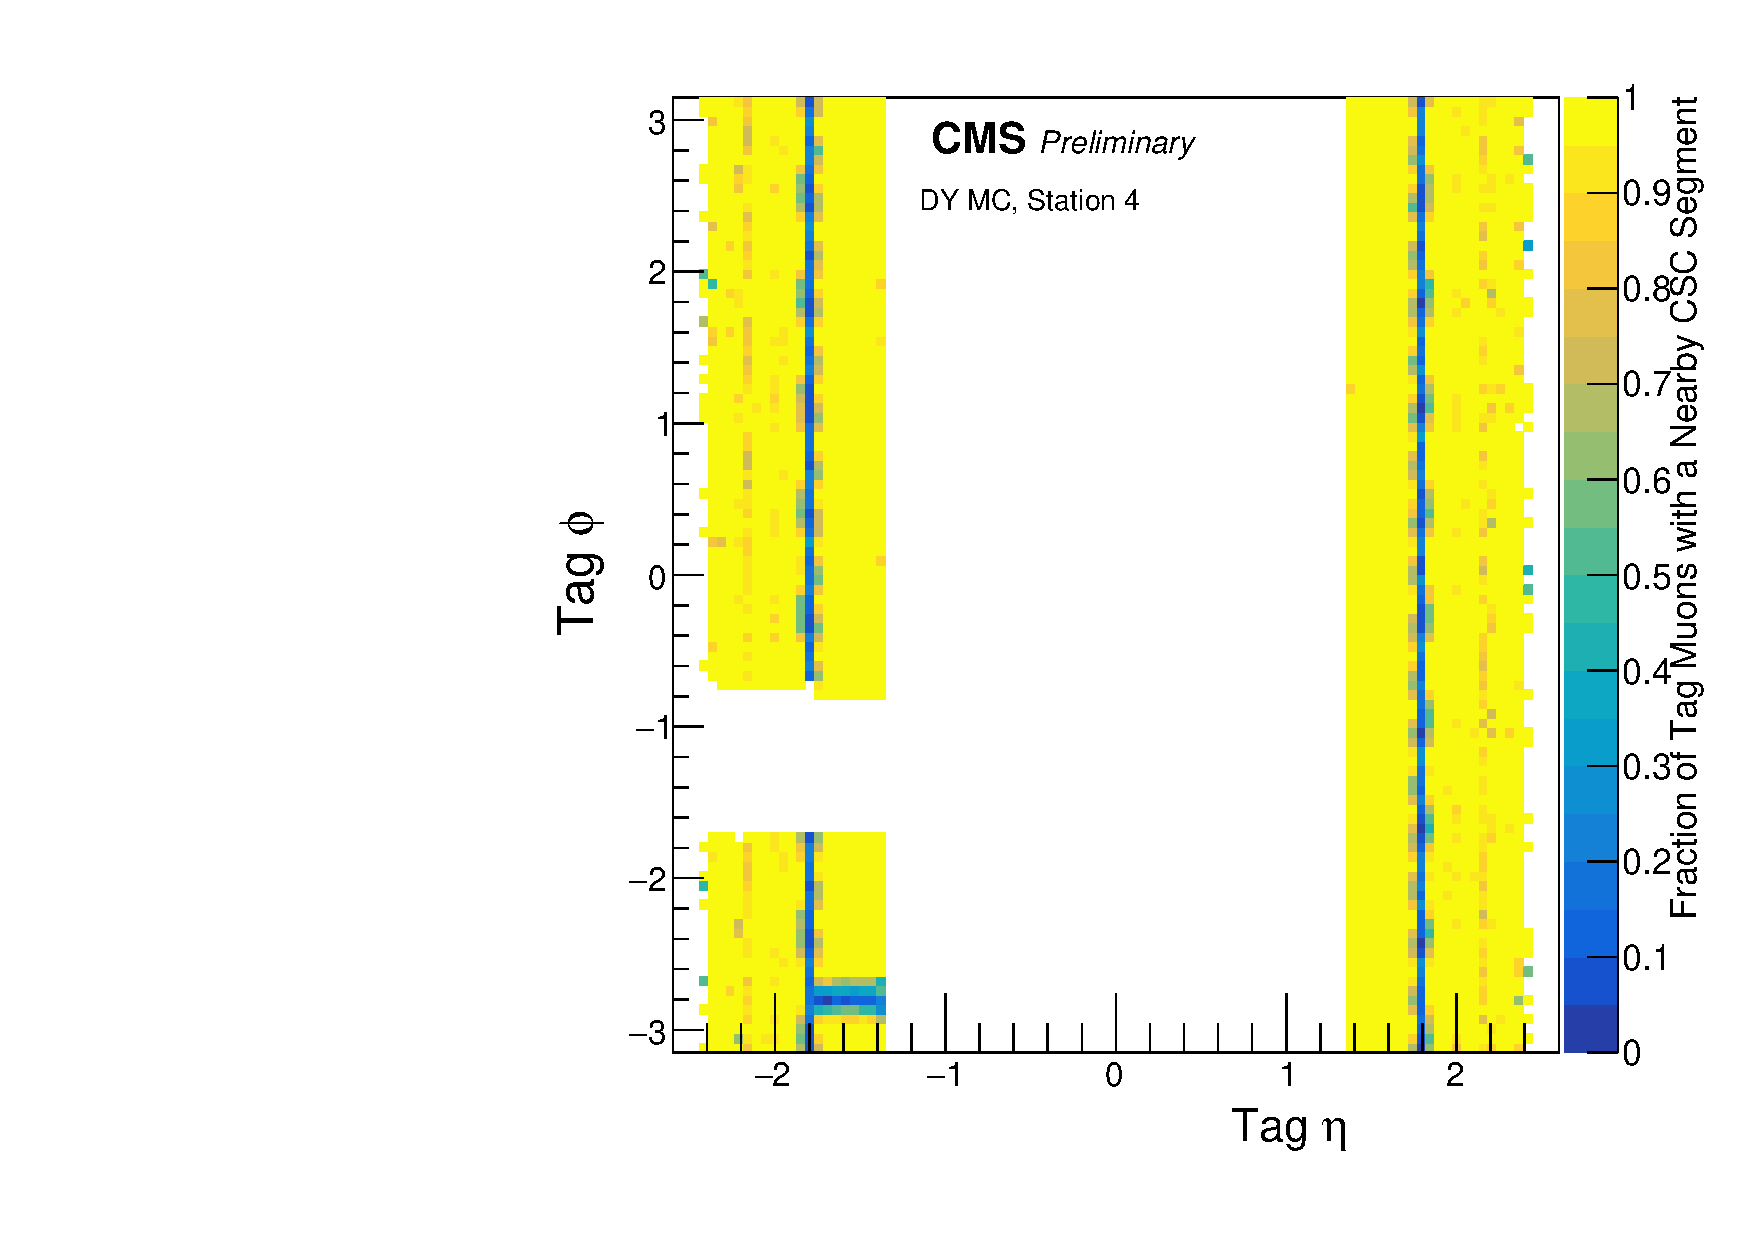
\includegraphics[width=0.45\textwidth]{figures/cscNearbyFracMC_station3.pdf}
    \caption[CSC segment efficiencies for stations three and four]{The fraction of tag muons with nearby CSC hits in the third and fourth CSC stations for data and MC. The lines of inefficient reconstruction near $|\eta|$=1.7 are produced by gaps in the CSCs which are designed to be non-projective across stations.}
    \label{fig:CSCeff2}
\end{figure}

To correct for these differences, simulated events which have only one nearby CSC segment are counted as complete disappearance events with weights proportional to the difference in efficiency for the CSC station and location where the segment was observed to represent the fraction of events that were reconstructed in MC but should have failed reconstruction in data.
These corrections increase the expected muon background rate by 22$\%$, and their uncertainties are dominated by the statistical uncertainty resulting from the sample size of simulated DY events with one or fewer nearby CSC segments.
Events with multiple nearby CSC segments are not included in this correction as the product of the CSC efficiency differences across multiple CSC stations reduces the impact below the 1$\%$ level, significantly smaller than the overall uncertainty of the expected background.

Using this simulation, 10.1$\pm$3 missed muon events are predicted in the complete disappearance category for the full 59.8$\fbinv$ of Run 2. 
This background prediction accounts for backgrounds both from failed reconstruction and hard bremsstrahlung or other scattering processes, and relies on the accuracy of the muon scattering in simulation which are validated using studies of the high-HCAL control region and HE hits aligned with tagging muons.

\subsection{Partial Disappearance Muon Backgrounds}
While the requirements of no nearby Standalone muons, CSC segments, or RPC hits are sufficient in the complete disappearance region to reduce muon backgrounds to a manageable level, the missing energy requirement (standalone muon energy $<$40$\%$ of probe track energy) alone still results in roughly 200,000 selected DY muons due to the relatively poor resolution of the standalone muon reconstruction.
To reduce this background, a binary decision tree is trained to separate potential signal events from muon backgrounds. 
The design, inputs, training, and validation of the BDT are described in detail in \Cref{sec:BDT}.

The expected muon background after applying the BDT selection is determined by scaling the BDT score distribution of simulated DY events to the total number of events which pass the base partial disappearance selection.
The resulting background prediction is thus directly dependent on this simulated BDT score distribution, which is validated using multiple control regions to compare the simulation of the input variables used and the resulting effect on the BDT score.
This validation is presented in \Cref{sec:BDTvalid}, and is used to calculate systematic uncertainties on the number of expected muon backgrounds resulting from differences in the simulated inputs and resulting BDT scores.

\section{Non-Muon Backgrounds}
Non-muon ("$\mu+X$") events occur when a tagging muon is paired with a probe track that does not originate from the decay of a Z boson. 
Non-muon tracks are very likely to be stopped by the calorimeters or to decay within them, mimicking signal events by having little or no ionization in the muon chambers. 
Unlike signal events, the interactions of these backgrounds in the calorimeters should produce visible energy deposits which can be used to reject the event.
Most importantly, $\mu+X$ events will not have a sharp peak in the tag/probe invariant mass like signal.
Because of this, control regions with inverted invariant mass selections can be defined which are composed nearly entirely of $\mu+X$ events to observe their properties, and simultaneous fits of the invariant mass to peaking and non-peaking functions can be performed in the signal regions allowing for entirely data-driven estimations of the background rate.

Among the possible particles which may produce the misidentified probe tracks, of particular interest are charged mesons such as pions or kaons, SM particles consisting of bound quark pairs which may decay into a muon and neutrino pair as they pass through the detector.
These mesons can be produced in the initial CMS collision, and would produce ionization in the tracker similarly to muons.
As the neutrinos produced in these meson decays are not visible in the detector, these decaying charged mesons could appear very similar to signal events, with the misidentified meson acting as the initial muon and the muon produced in the decay acting as a deflected muon with energy loss to a neutrino instead of a dark photon.

The overall rate of these meson backgrounds is reduced by several factors.
The initial meson must decay within the detector to a signal-like final state, and must do so before undergoing significant showering in the detector.
The typical branching fractions to final states with muons and neutrinos and the relatively long lifetimes of these mesons, along with their Lorentz boosts when decaying in the lab frame, produce decay rates within the detector on the order of 0.1$\%$ for most mesons without accounting for interactions with the detector.
Mesons are likely to produce showers in the ECAL or HCAL before decaying, increasing their likelihood to fail the isolation requirements and reducing the rate of their selection.

The low mass of the neutrino favors the muon carrying most of the outgoing momentum in the collision, so that only a small fraction of meson decays result in significant energy differences between the outgoing muon and the initial meson.
Lastly, mesons produced in the collision are rarely isolated, and are generally produced in jets of particles which are likely to cause the event to fail the isolation selections through their own tracks and deposits in the calorimeters.

While $\mu+X$ backgrounds specifically refer to events where the selected probe track does not match to a muon produced in the DY process, DY$\rightarrow\mu\mu$ events can contribute to this region when one muon is reconstructed well and is used as the tag while the other is out of detector acceptance or fails both track and standalone muon reconstruction such that it does not pass the tag/probe pairing requirements. 
In these cases, an un-associated track may be selected as the probe and a non-muon background can be produced from a DY$\rightarrow\mu\mu$ event. 
This corresponds to roughly 5$\%$ of the expected $\mu$+X background.

The properties of $\mu+X$ events are observed using control regions of events with invariant masses far from the Z-peak or with tag/probe pairs that have same-sign charges.
In both signal regions, the off-peak events are fit with a non-peaking function to predict the nominal background in the signal region, and the same-sign control region is used to validate assumptions of the background shape.
In the complete disappearance region, the off-peak events are also used to set the threshold used for HCAL isolation by optimizing the signal strength of the final fit as a function of isolation and the resulting expected $\mu$+X background and signal efficiency.

For the final simultaneous fits in the complete disappearance region, the $\mu+X$ background is fit using a non-peaking background with nominal fit shape and amplitude from the off-peak control regions, and the combined signal and muon backgrounds are fit using the DY invariant mass shape determined from data events in order to account for potential inaccuracies in the simulated DY invariant mass distribution.
Events used to find this shape are selected using events with two tight-ID muons which otherwise pass the kinematic, pairing, and isolation requirements used for the base event selection, and a shape uncertainty of $\pm$1 GeV is applied which shifts the peak location of the invariant mass to account for potential bias from the energy dependence of the signal interaction.

In the partial disappearance region, the low rate of $\mu+X$ backgrounds compared to DY backgrounds prevents effective fitting of the two shapes, and so a single bin fit is performed using the expected number of $\mu+X$ events from the off-peak region and the number of DY events expected from simulation.

\subsection{Off Peak Control Region}
In the off-peak control region, the full signal selections are applied with the invariant mass requirement inverted to be far from the Z-peak ($50<M_{\mu\mu}<70$ or $110<M_{\mu\mu}<150$ \GeV). 
The resulting region contains very little DY contribution due to the strongly peaking shape of DY events, resulting in a very pure sample of $\mu+X$ background events. 
By fitting the off-peak region using a non-peaking background function (\Cref{eq:bkgfunc}) derived using a control region of poorly isolated probe tracks, the expected $\mu+X$ rate in the signal region can be predicted entirely from data. 
The results of this fit for data events in the complete disappearance off-peak events as well as data and MC events without HCAL or ECAL isolation requirements is shown in \Cref{fig:offpeakfit}.

\begin{equation} 
    \label{eq:bkgfunc}
    f(s)=A+B(s-C)e^{-Ds} 
\end{equation}

\begin{figure}[htp]
    \centering
    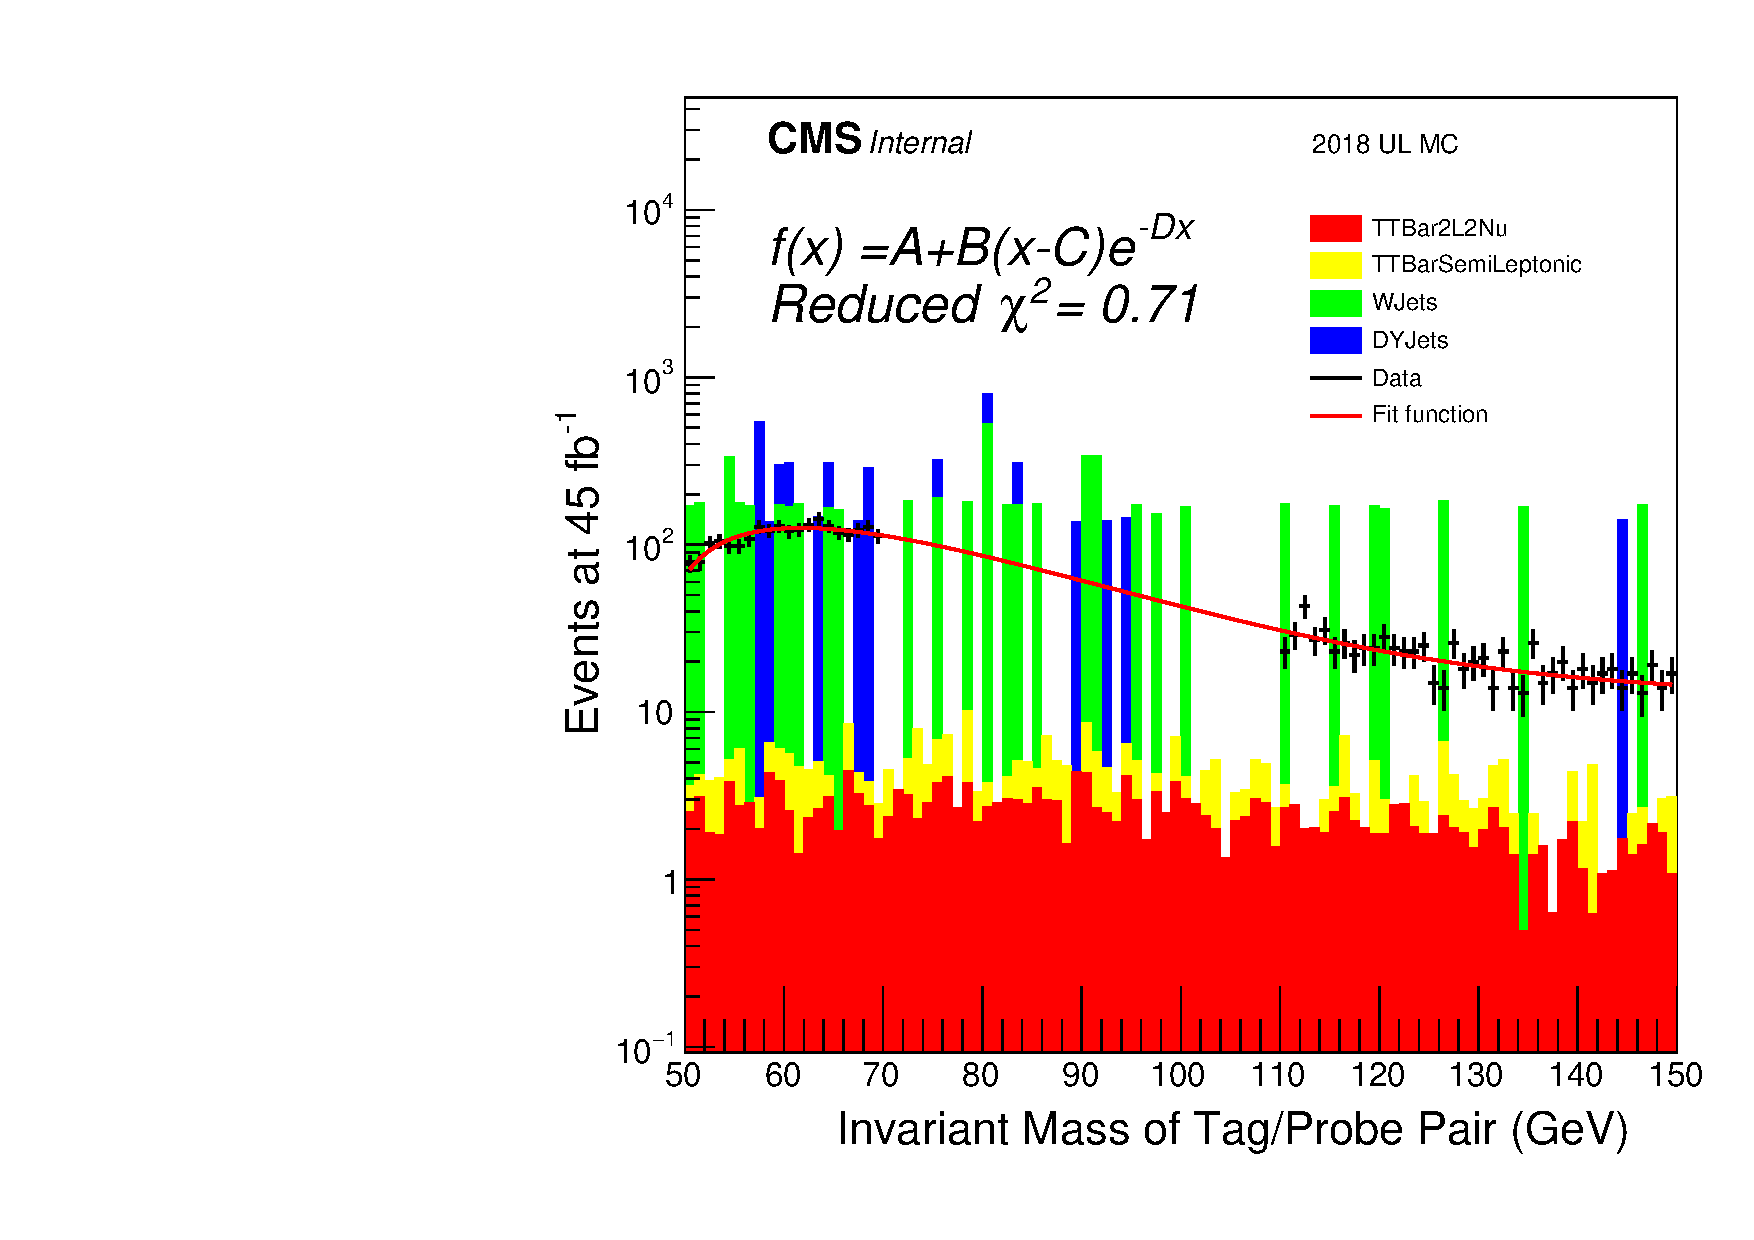
\includegraphics[width=0.45\textwidth]{figures/offPeakCr_noIso.pdf}
    \hspace{0.01\textwidth}
    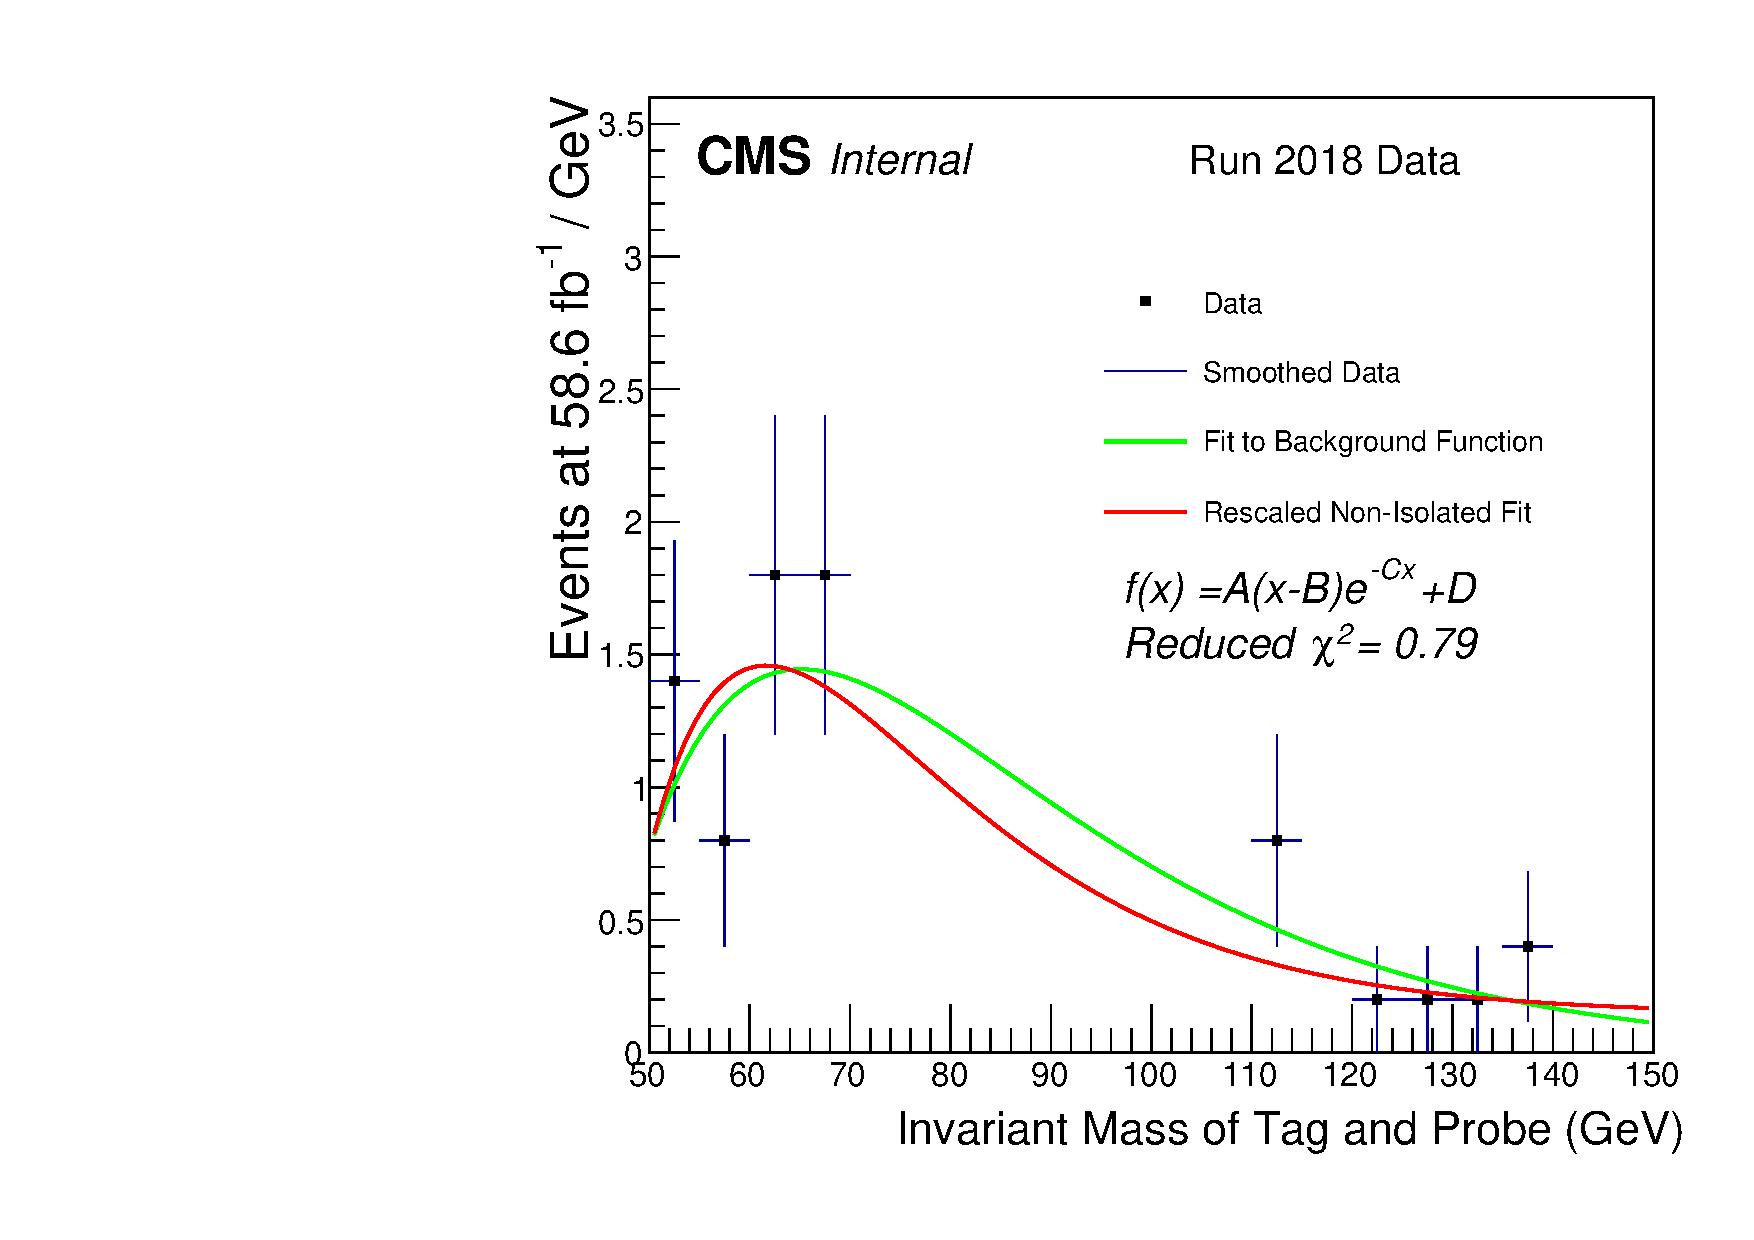
\includegraphics[width=0.45\textwidth]{figures/offPeakCr_fit.pdf} 
     \caption[$\mu$+X background fits in the off-peak control region for complete disappearance events]{The invariant mass distribution in the signal region without HCAL isolation requirements for data and MC (left), and the complete disappearance off-peak control region fit in data (right).}
    \label{fig:offpeakfit}
 \end{figure}
 
This fit is then used to predict the nominal $\mu+$X background amplitude in the complete disappearance region, but is dependent on the chosen functional form. 
Two separate fits are performed - one 'free' fit which directly uses the background function, and one which first fits data events in the non-isolated region and then re-scales the result to the isolated region. 
The re-scaled fit has less statistical uncertainty due to the larger sample size in the non-isolated region, but does not include any potential changes in shape due to applying the isolation requirements. 
The free fit results in a 15$\%$ larger expected background than the re-scaled fit. 
The re-scaled fit is taken as the central value of the predicted yield, and the difference between the two is applied to the signal region fit as a shape uncertainty.

In partial disappearance events, the requirement of nearby standalone muons greatly reduces the rate of $\mu+X$ backgrounds, resulting in very low occupancy in the off-peak region. 
In addition, the high rate of expected DY backgrounds combined with the width of the Z-peak results in two expected DY background events in the off-peak region, shifting the expected distribution away from the nominal non-peaking function.

Because of the poor fit quality for the non-peaking background function resulting from the low occupancy and DY contamination, the alternate fit function used in this region is a constant value.
Data events in the off-peak partial disappearance region, along with fits to the non-peaking background function and a constant value, are shown in \Cref{fig:offPeakPartialDis}.
The inclusion of the DY contribution in the off-peak fit and the resulting non-Z background prediction results in a small decrease in the signal sensitivity.
Due to the much larger rate of DY backgrounds than $\mu+X$ backgrounds, this decrease in sensitivity is $<$1$\%$.

\begin{figure}[htp]
    \centering
    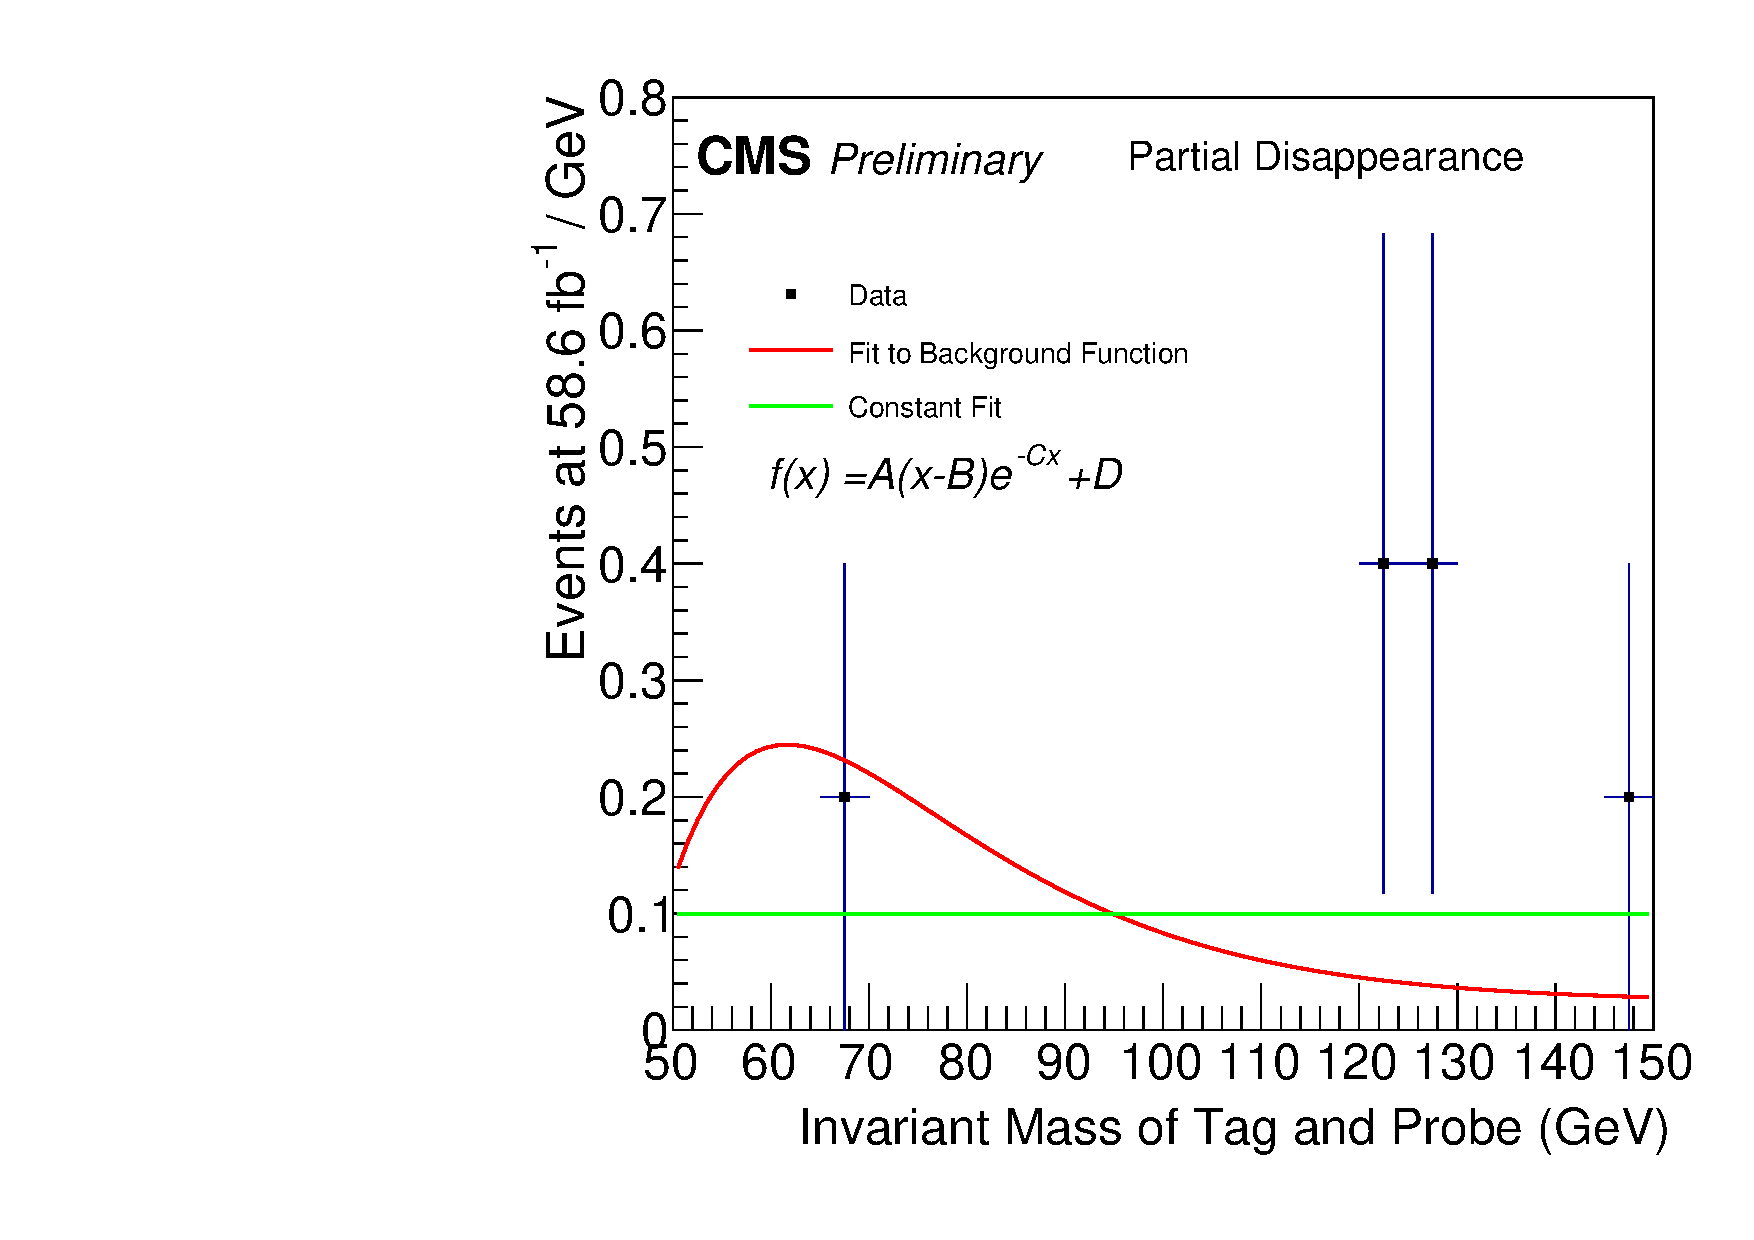
\includegraphics[width=0.45\textwidth]{figures/offPeakFitPartialDisappearance.pdf}
     \caption[$\mu$+X background fits in the off-peak control region for partial disappearance events]{The partial disappearance off-peak control region in data, as well as fits to the non-peaking background function and an alternate fit to a constant value. Events with invariant masses between 70 and 110 GeV are explicitly excluded from the control region as well as the fits.}
    \label{fig:offPeakPartialDis}
 \end{figure}

\subsection{Non-Muonic Z decays}
The core assumption used in predicting the rate of $\mu$+X backgrounds with data is that their tag and probe invariant mass distributions follow some smooth function which does not peak near the Z-mass or have significant shape differences to the fit functions used.
Conceptually, a source of $\mu$+X backgrounds which could have peaking invariant mass distributions which may not be effectively fit by the off-peak control region are Z bosons which decay to hadrons or $\tau$ leptons.
These events can produce potentially dangerous backgrounds in cases where one $\tau$ decays leptonically and produces a good tag muon, while the other might decay into a pion or other particle which fakes a probe muon. 

While the invariant mass of the initially produced $\tau$ leptons or hadrons is near the Z mass, the final state muons or mesons which are selected in this search are expected to have substantially shifted invariant mass distributions due to only selecting a portion of the produced particles, as $\tau$ or hadron decays which produce the selected muons will also produce some number of other particles which carry some of the initial energy.
Simulated DY events which match the selected probes to generated $\tau$ leptons or hadrons are used to confirm that they do not produce an invariant mass peak within the signal region.

Because of the very low rate of these events passing the probe isolation requirements, the invariant mass distributions are measured without applying track or ECAL isolation requirements.
The invariant mass of selected tag and probe pairs from Z decays to $\tau$ leptons or hadrons in MC without the full isolation selections applied is shown in \Cref{fig:ZtoTauTau}.
As expected, the additional particles produced in hadronic and $\tau$ decays of the Z boson shift the invariant mass of the tag and probe such that there is no longer a peak near the Z mass, and these potential background sources are effectively included by the non-peaking $\mu$+X fit.

\begin{figure}[htp]
    \centering
    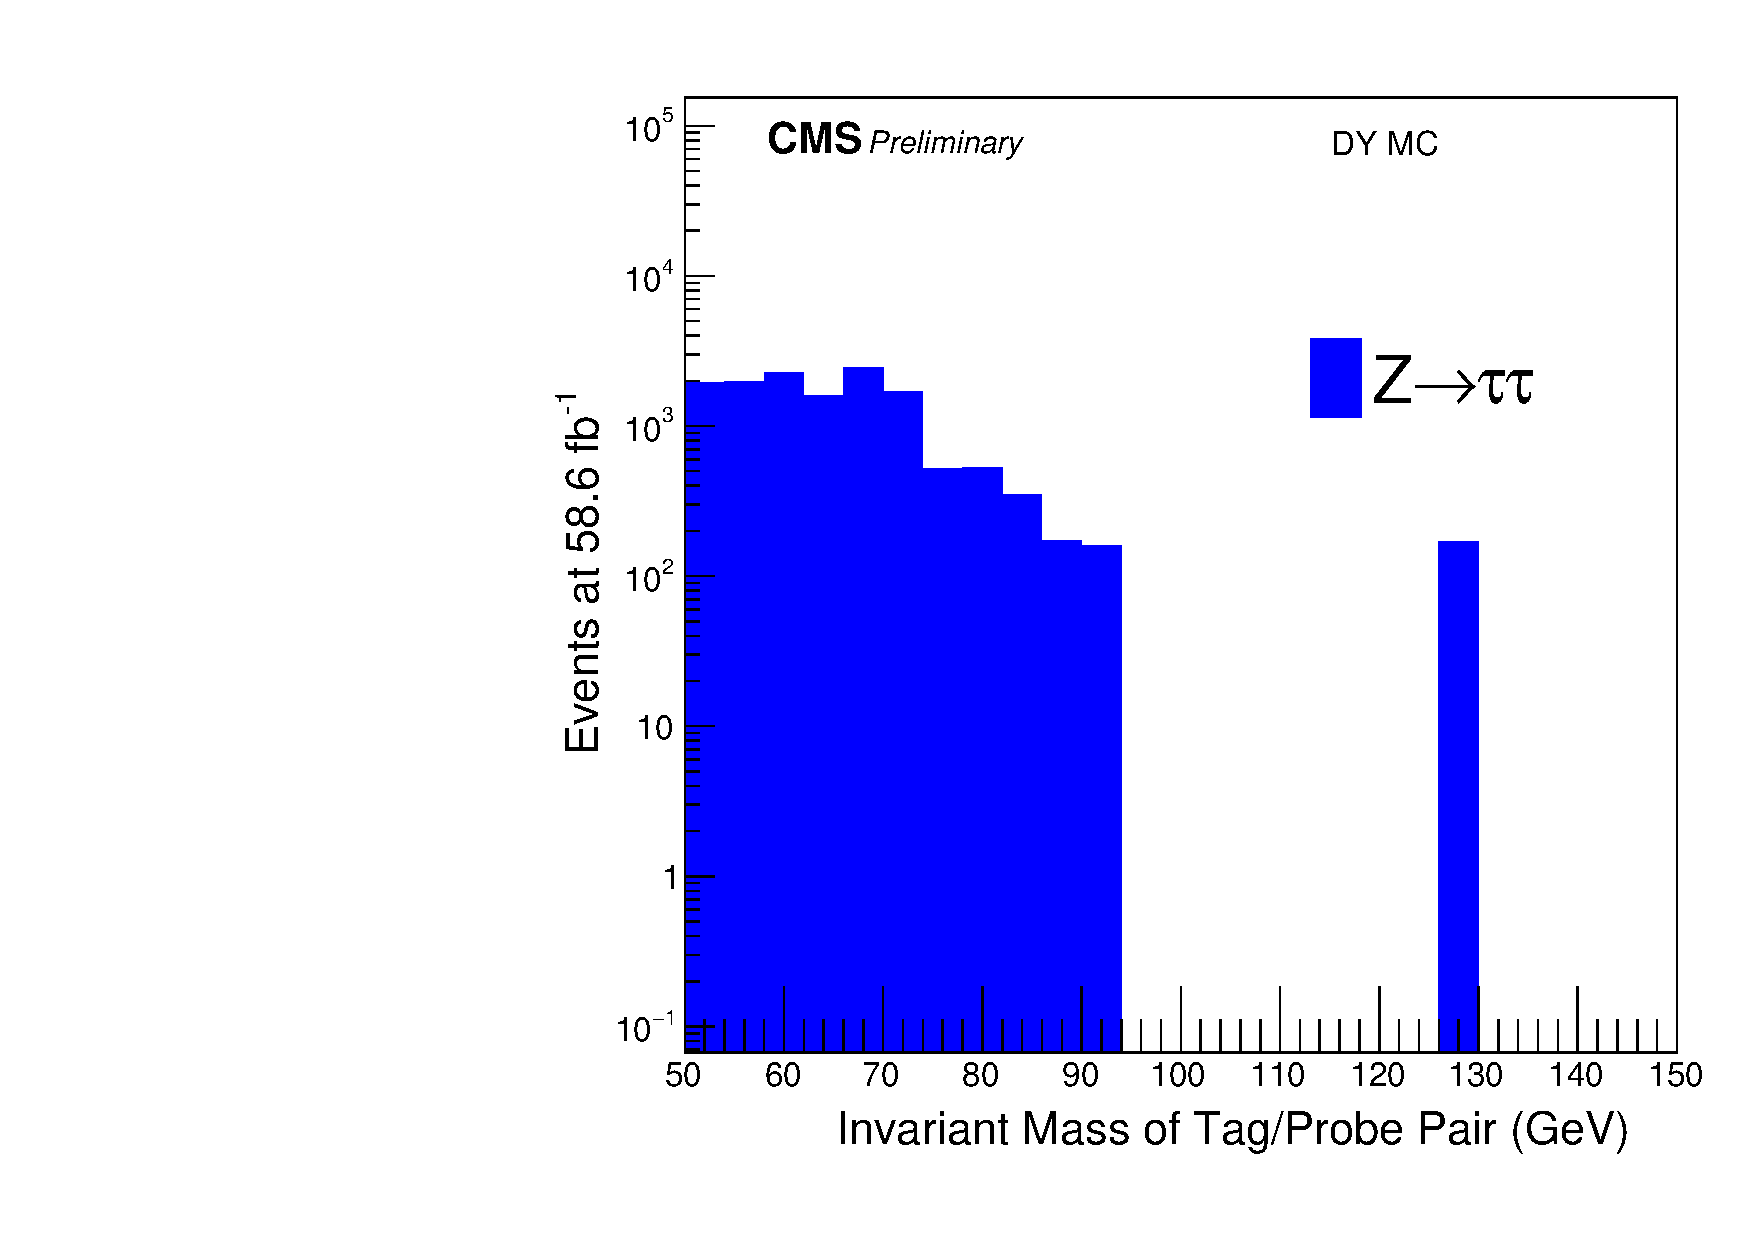
\includegraphics[width=0.45\textwidth]{figures/tauZInvMass.pdf}
    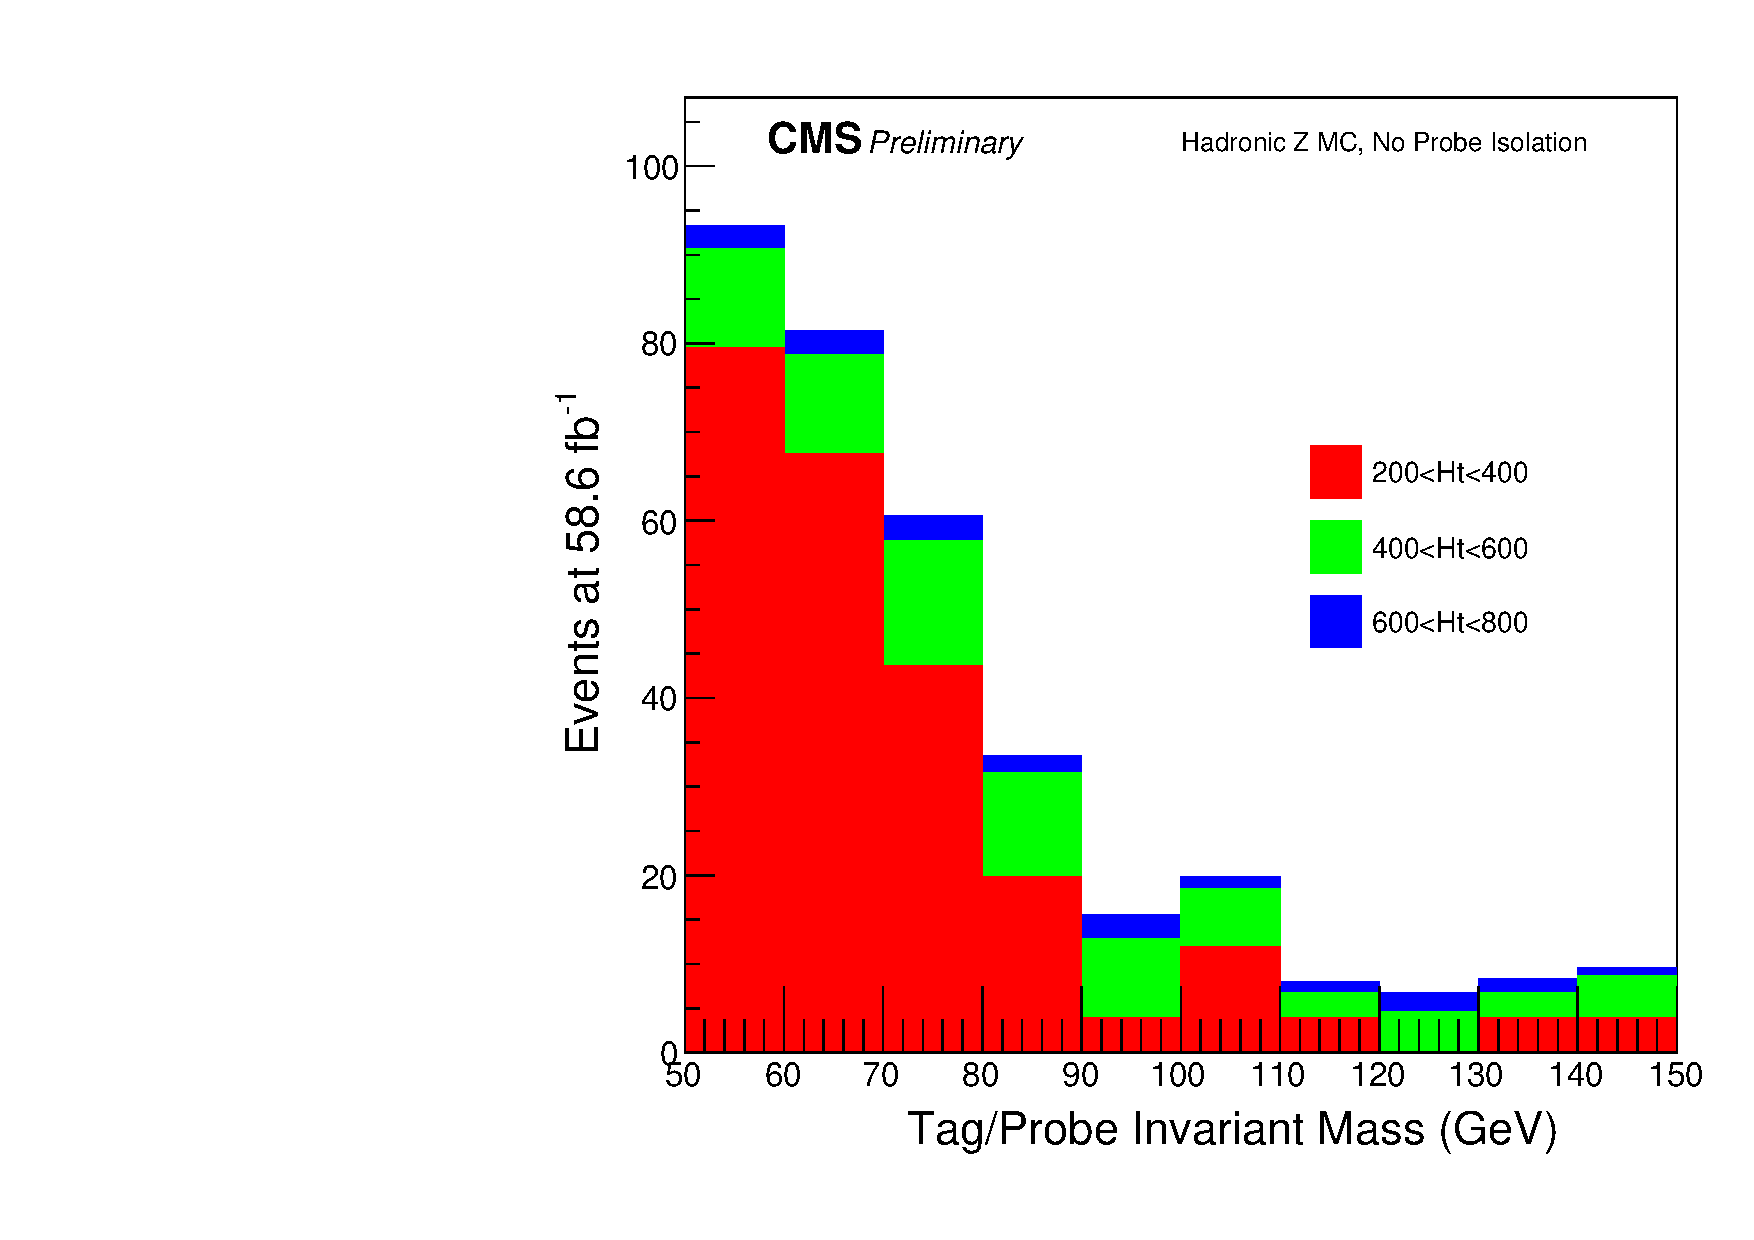
\includegraphics[width=0.45\textwidth]{figures/hadronZInvMass.pdf}
     \caption[The invariant mass of hadronic and $\tau$ Z decays]{The invariant mass distributions of DY events which match gen level $\tau$ leptons to the selected probes (left) and hadronic Z decays (right). Neither background process has a significant peak within the signal region, and they should therefore be included effectively in the off peak control region fits.}
    \label{fig:ZtoTauTau}
\end{figure}

\section{Signal Contamination}
\label{sec:SigContamination}
While the control regions used are generally chosen to contain as few signal events as possible, the requirements applied are not perfectly efficient and some signal rate is still present within them.
This effect, referred to as signal contamination, can have several impacts on the measured result depending on the amount of signal present and the control regions in which it is found.

In the off-peak control region, signal contamination could potentially increase the predicted $\mu+X$ background by being included in the non-peaking fit. 
Using the functional form of the off-peak fit used in Figure \ref{fig:offpeakfit}, each signal event in the off-peak control region fit will add 0.5 expected $\mu+X$ events to the background prediction in the signal region.

In partial disappearance events the single-bin fit results in these additional events directly contributing to the expected background and therefore reducing the signal sensitivity. 
In complete disappearance events ,the off-peak prediction is only used to predict the nominal $\mu$+X scale, and the simultaneous fit within the signal region reduces the impact of signal contamination by exploiting the shape difference between $\mu$+X and signal or DY events.

Because of the strongly peaking nature of the invariant mass in signal events, one signal event is expected to appear in the off-peak region for every 20 events in the signal region.
Combining the effects of the off-peak fit extrapolation and the invariant mass shape, the expected signal contamination in the off-peak control region would reduce the signal sensitivity by at most $2.5\%$ for all signal masses and regions.

In the hard Bremsstrahlung control region, events are selected which have large HCAL energy along the probe track trajectory in order to validate the simulation of MC events with visible energy deposits from standard model Bremsstrahlung, as well as to test the partial disappearance BDT classification using data. 
As the difference in the BDT shape between data and MC in this region is used to derive a systematic uncertainty on the BDT shape of DY backgrounds, extra high-scoring events from signal contamination would increase this uncertainty and reduce the final signal sensitivity.

There are several factors which reduce the impact of this effect.
Signal events are less likely to have high-energy SM interactions before producing dark matter, as reductions in the muon energy lower the production cross section of dark bremsstrahlung.
Signal events are also less likely to deposit large amounts of energy in HE after a dark matter interaction, as the low energy of outgoing muons reduces the energy available for SM Bremsstrahlung. 

In addition, DY events in the hard Bremsstrahlung control region appear much more background-like than in the signal region due to energy loss from SM processes.
DY background events pass the BDT score requirement of $>0.98$ much more frequently in the high-HCAL energy control region than the signal region, while signal events have similar BDT score distributions in both regions. 
The combination of these effects results in an expected signal loss of 4$\%$ from signal contamination in the corrections derived in the high-HCAL energy region.
